\documentclass[12pt]{beamer}\usepackage[]{graphicx}\usepackage[]{color}
%% maxwidth is the original width if it is less than linewidth
%% otherwise use linewidth (to make sure the graphics do not exceed the margin)
\makeatletter
\def\maxwidth{ %
  \ifdim\Gin@nat@width>\linewidth
    \linewidth
  \else
    \Gin@nat@width
  \fi
}
\makeatother

\definecolor{fgcolor}{rgb}{0.345, 0.345, 0.345}
\newcommand{\hlnum}[1]{\textcolor[rgb]{0.686,0.059,0.569}{#1}}%
\newcommand{\hlstr}[1]{\textcolor[rgb]{0.192,0.494,0.8}{#1}}%
\newcommand{\hlcom}[1]{\textcolor[rgb]{0.678,0.584,0.686}{\textit{#1}}}%
\newcommand{\hlopt}[1]{\textcolor[rgb]{0,0,0}{#1}}%
\newcommand{\hlstd}[1]{\textcolor[rgb]{0.345,0.345,0.345}{#1}}%
\newcommand{\hlkwa}[1]{\textcolor[rgb]{0.161,0.373,0.58}{\textbf{#1}}}%
\newcommand{\hlkwb}[1]{\textcolor[rgb]{0.69,0.353,0.396}{#1}}%
\newcommand{\hlkwc}[1]{\textcolor[rgb]{0.333,0.667,0.333}{#1}}%
\newcommand{\hlkwd}[1]{\textcolor[rgb]{0.737,0.353,0.396}{\textbf{#1}}}%

\usepackage{framed}
\makeatletter
\newenvironment{kframe}{%
 \def\at@end@of@kframe{}%
 \ifinner\ifhmode%
  \def\at@end@of@kframe{\end{minipage}}%
  \begin{minipage}{\columnwidth}%
 \fi\fi%
 \def\FrameCommand##1{\hskip\@totalleftmargin \hskip-\fboxsep
 \colorbox{shadecolor}{##1}\hskip-\fboxsep
     % There is no \\@totalrightmargin, so:
     \hskip-\linewidth \hskip-\@totalleftmargin \hskip\columnwidth}%
 \MakeFramed {\advance\hsize-\width
   \@totalleftmargin\z@ \linewidth\hsize
   \@setminipage}}%
 {\par\unskip\endMakeFramed%
 \at@end@of@kframe}
\makeatother

\definecolor{shadecolor}{rgb}{.97, .97, .97}
\definecolor{messagecolor}{rgb}{0, 0, 0}
\definecolor{warningcolor}{rgb}{1, 0, 1}
\definecolor{errorcolor}{rgb}{1, 0, 0}
\newenvironment{knitrout}{}{} % an empty environment to be redefined in TeX

\usepackage{alltt}
\usepackage{graphicx}
\usepackage{tikz}
\setbeameroption{hide notes}
\setbeamertemplate{note page}[plain]
\usepackage{listings}

% get rid of junk
\usetheme{default}
\usefonttheme[onlymath]{serif}
\beamertemplatenavigationsymbolsempty
\hypersetup{pdfpagemode=UseNone} % don't show bookmarks on initial view

% named colors
\definecolor{offwhite}{RGB}{255,250,240}
\definecolor{gray}{RGB}{155,155,155}

\ifx\notescolors\undefined % slides

  \definecolor{foreground}{RGB}{80,80,80}
  \definecolor{background}{RGB}{255,255,255}
  \definecolor{title}{RGB}{255,199,0}
  \definecolor{subtitle}{RGB}{89,132,212}
  \definecolor{hilit}{RGB}{248,117,79}
  \definecolor{vhilit}{RGB}{255,111,207}
  \definecolor{lolit}{RGB}{200,200,200}
  \definecolor{lit}{RGB}{255,199,0}
  \definecolor{mdlit}{RGB}{89,132,212}
  \definecolor{link}{RGB}{248,117,79}

\else % notes
  \definecolor{background}{RGB}{255,255,255}
  \definecolor{foreground}{RGB}{24,24,24}
  \definecolor{title}{RGB}{27,94,134}
  \definecolor{subtitle}{RGB}{22,175,124}
  \definecolor{hilit}{RGB}{122,0,128}
  \definecolor{vhilit}{RGB}{255,0,128}
  \definecolor{lolit}{RGB}{95,95,95}
\fi
\definecolor{nhilit}{RGB}{128,0,128}  % hilit color in notes
\definecolor{nvhilit}{RGB}{255,0,128} % vhilit for notes

\newcommand{\hilit}{\color{hilit}}
\newcommand{\vhilit}{\color{vhilit}}
\newcommand{\nhilit}{\color{nhilit}}
\newcommand{\nvhilit}{\color{nvhilit}}
\newcommand{\lit}{\color{lit}}
\newcommand{\mdlit}{\color{mdlit}}
\newcommand{\lolit}{\color{lolit}}

% use those colors
\setbeamercolor{titlelike}{fg=title}
\setbeamercolor{subtitle}{fg=subtitle}
\setbeamercolor{frametitle}{fg=gray}
\setbeamercolor{structure}{fg=subtitle}
\setbeamercolor{institute}{fg=lolit}
\setbeamercolor{normal text}{fg=foreground,bg=background}
%\setbeamercolor{item}{fg=foreground} % color of bullets
%\setbeamercolor{subitem}{fg=hilit}
%\setbeamercolor{itemize/enumerate subbody}{fg=lolit}
\setbeamertemplate{itemize subitem}{{\textendash}}
\setbeamerfont{itemize/enumerate subbody}{size=\footnotesize}
\setbeamerfont{itemize/enumerate subitem}{size=\footnotesize}

% center title of slides
\setbeamertemplate{blocks}[rounded]
\setbeamertemplate{frametitle}[default][center]
% margins
\setbeamersize{text margin left=25pt,text margin right=25pt}

% page number
\setbeamertemplate{footline}{%
    \raisebox{5pt}{\makebox[\paperwidth]{\hfill\makebox[20pt]{\lolit
          \scriptsize\insertframenumber}}}\hspace*{5pt}}

% add a bit of space at the top of the notes page
\addtobeamertemplate{note page}{\setlength{\parskip}{12pt}}

% default link color
\hypersetup{colorlinks, urlcolor={link}}

\ifx\notescolors\undefined % slides
  % set up listing environment
  \lstset{language=bash,
          basicstyle=\ttfamily\scriptsize,
          frame=single,
          commentstyle=,
          backgroundcolor=\color{darkgray},
          showspaces=false,
          showstringspaces=false
          }
\else % notes
  \lstset{language=bash,
          basicstyle=\ttfamily\scriptsize,
          frame=single,
          commentstyle=,
          backgroundcolor=\color{offwhite},
          showspaces=false,
          showstringspaces=false
          }
\fi

% a few macros
\newcommand{\code}[1]{\texttt{#1}}
\newcommand{\hicode}[1]{{\hilit \texttt{#1}}}
\newcommand{\bb}[1]{\begin{block}{#1}}
\newcommand{\eb}{\end{block}}
\newcommand{\bi}{\begin{itemize}}
%\newcommand{\bbi}{\vspace{24pt} \begin{itemize} \itemsep8pt}
\newcommand{\bbi}{\vspace{4pt} \begin{itemize} \itemsep8pt}
\newcommand{\ei}{\end{itemize}}
\newcommand{\bv}{\begin{verbatim}}
\newcommand{\ev}{\end{verbatim}}
\newcommand{\ig}{\includegraphics}
\newcommand{\subt}[1]{{\footnotesize \color{subtitle} {#1}}}
\newcommand{\ttsm}{\tt \small}
\newcommand{\ttfn}{\tt \footnotesize}
\newcommand{\figh}[2]{\centerline{\includegraphics[height=#2\textheight]{#1}}}
\newcommand{\figw}[2]{\centerline{\includegraphics[width=#2\textwidth]{#1}}}



%------------------------------------------------
% end of header
%------------------------------------------------

\title{Graphics in R}
\subtitle{STAT 133}
\author{\href{http://www.gastonsanchez.com}{Gaston Sanchez}}
\institute{Department of Statistics, UC{\textendash}Berkeley}
\date{\href{http://www.gastonsanchez.com}{\tt \scriptsize \color{foreground} gastonsanchez.com}
\\[-4pt]
\href{http://github.com/gastonstat/stat133}{\tt \scriptsize \color{foreground} github.com/gastonstat/stat133}
\\[-4pt]
{\scriptsize Course web: \href{http://www.gastonsanchez.com/stat133}{\tt gastonsanchez.com/stat133}}
}
\IfFileExists{upquote.sty}{\usepackage{upquote}}{}
\begin{document}


{
  \setbeamertemplate{footline}{} % no page number here
  \frame{
    \titlepage
  } 
}

%------------------------------------------------

\begin{frame}
\begin{center}
\Huge{\hilit{Base Graphics}}
\end{center}
\end{frame}

%------------------------------------------------

\begin{frame}
\frametitle{Graphics in R}

\bb{Traditional Graphics}
\bi
  \item R \code{"graphics"} follows a static, "painting on canvas" model.
  \item Graphics elements are drawn, and remain visible until painted over.
  \item For dynamic and/or interactive graphics, R is limited.
\ei
\eb

\end{frame}

%------------------------------------------------

\begin{frame}
\frametitle{Traditional Graphics}

\bb{Traditional graphics model}
In the traditional model, we create a plot by first calling a high-level function that creates a complete plot, and then we call low-level functions to add more output if necessary
\eb

\end{frame}

%------------------------------------------------

\begin{frame}[fragile]
\frametitle{Dataset \code{mtcars}}
\begin{knitrout}\scriptsize
\definecolor{shadecolor}{rgb}{0.969, 0.969, 0.969}\color{fgcolor}\begin{kframe}
\begin{alltt}
\hlkwd{head}\hlstd{(mtcars)}
\end{alltt}
\begin{verbatim}
##                    mpg cyl disp  hp drat    wt  qsec vs am gear carb
## Mazda RX4         21.0   6  160 110 3.90 2.620 16.46  0  1    4    4
## Mazda RX4 Wag     21.0   6  160 110 3.90 2.875 17.02  0  1    4    4
## Datsun 710        22.8   4  108  93 3.85 2.320 18.61  1  1    4    1
## Hornet 4 Drive    21.4   6  258 110 3.08 3.215 19.44  1  0    3    1
## Hornet Sportabout 18.7   8  360 175 3.15 3.440 17.02  0  0    3    2
## Valiant           18.1   6  225 105 2.76 3.460 20.22  1  0    3    1
\end{verbatim}
\end{kframe}
\end{knitrout}
\end{frame}

%------------------------------------------------

\begin{frame}[fragile]
\frametitle{Scatter plot}
\begin{knitrout}\footnotesize
\definecolor{shadecolor}{rgb}{0.969, 0.969, 0.969}\color{fgcolor}\begin{kframe}
\begin{alltt}
\hlcom{# simple scatter-plot}
\hlkwd{plot}\hlstd{(mtcars}\hlopt{$}\hlstd{mpg, mtcars}\hlopt{$}\hlstd{hp)}
\end{alltt}
\end{kframe}

{\centering 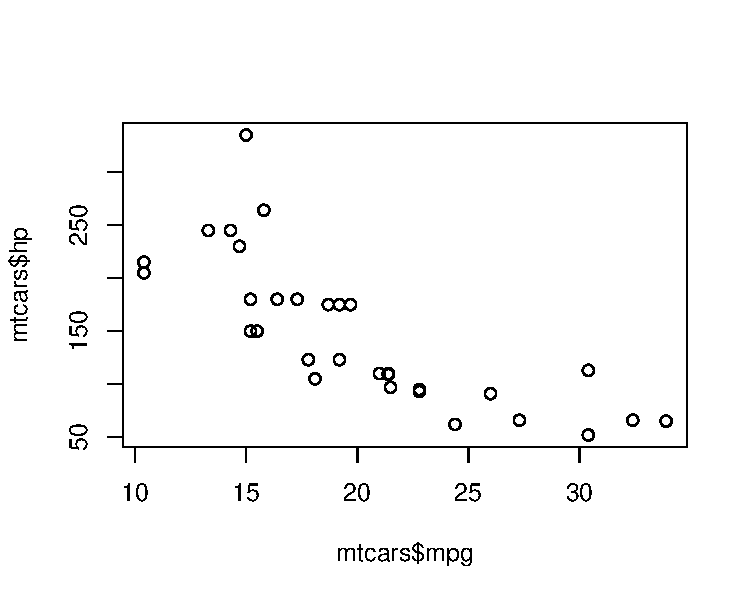
\includegraphics[width=.65\linewidth,height=.55\linewidth]{figure/unnamed-chunk-2-1} 

}



\end{knitrout}
\end{frame}

%------------------------------------------------

\begin{frame}[fragile]
\frametitle{Axis Labels}
\begin{knitrout}\scriptsize
\definecolor{shadecolor}{rgb}{0.969, 0.969, 0.969}\color{fgcolor}\begin{kframe}
\begin{alltt}
\hlcom{# xlab and ylab}
\hlkwd{plot}\hlstd{(mtcars}\hlopt{$}\hlstd{mpg, mtcars}\hlopt{$}\hlstd{hp,} \hlkwc{xlab} \hlstd{=} \hlstr{"miles per gallon"}\hlstd{,}
     \hlkwc{ylab} \hlstd{=} \hlstr{"horsepower"}\hlstd{)}
\end{alltt}
\end{kframe}

{\centering 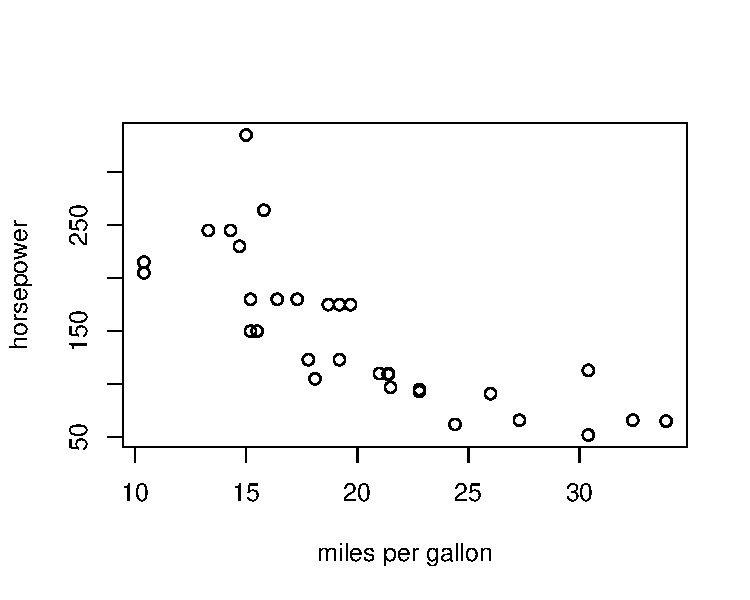
\includegraphics[width=.65\linewidth,height=.6\linewidth]{figure/unnamed-chunk-3-1} 

}



\end{knitrout}
\end{frame}

%------------------------------------------------

\begin{frame}[fragile]
\frametitle{Title and subtitle}
\begin{knitrout}\scriptsize
\definecolor{shadecolor}{rgb}{0.969, 0.969, 0.969}\color{fgcolor}\begin{kframe}
\begin{alltt}
\hlcom{# title and subtitle}
\hlkwd{plot}\hlstd{(mtcars}\hlopt{$}\hlstd{mpg, mtcars}\hlopt{$}\hlstd{hp,} \hlkwc{xlab} \hlstd{=} \hlstr{"miles per gallon"}\hlstd{,}
     \hlkwc{ylab} \hlstd{=} \hlstr{"horsepower"}\hlstd{,} \hlkwc{main} \hlstd{=} \hlstr{"Simple Scatterplot"}\hlstd{,}
     \hlkwc{sub} \hlstd{=} \hlstr{'data matcars'}\hlstd{)}
\end{alltt}
\end{kframe}

{\centering 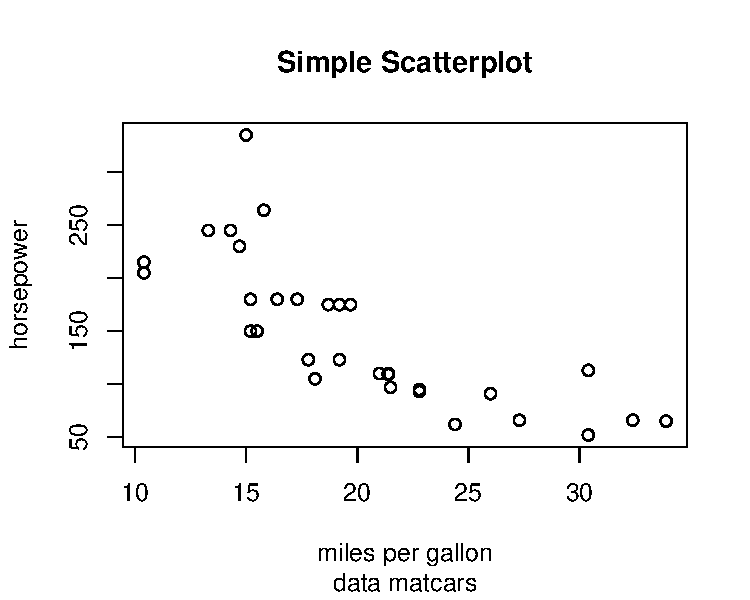
\includegraphics[width=.65\linewidth,height=.6\linewidth]{figure/unnamed-chunk-4-1} 

}



\end{knitrout}
\end{frame}

%------------------------------------------------

\begin{frame}[fragile]
\frametitle{x and y coordinate ranges}
\begin{knitrout}\scriptsize
\definecolor{shadecolor}{rgb}{0.969, 0.969, 0.969}\color{fgcolor}\begin{kframe}
\begin{alltt}
\hlcom{# 'xlim' and 'ylim'}
\hlkwd{plot}\hlstd{(mtcars}\hlopt{$}\hlstd{mpg, mtcars}\hlopt{$}\hlstd{hp,} \hlkwc{xlim} \hlstd{=} \hlkwd{c}\hlstd{(}\hlnum{10}\hlstd{,} \hlnum{35}\hlstd{),} \hlkwc{ylim} \hlstd{=} \hlkwd{c}\hlstd{(}\hlnum{50}\hlstd{,} \hlnum{400}\hlstd{))}
\end{alltt}
\end{kframe}

{\centering 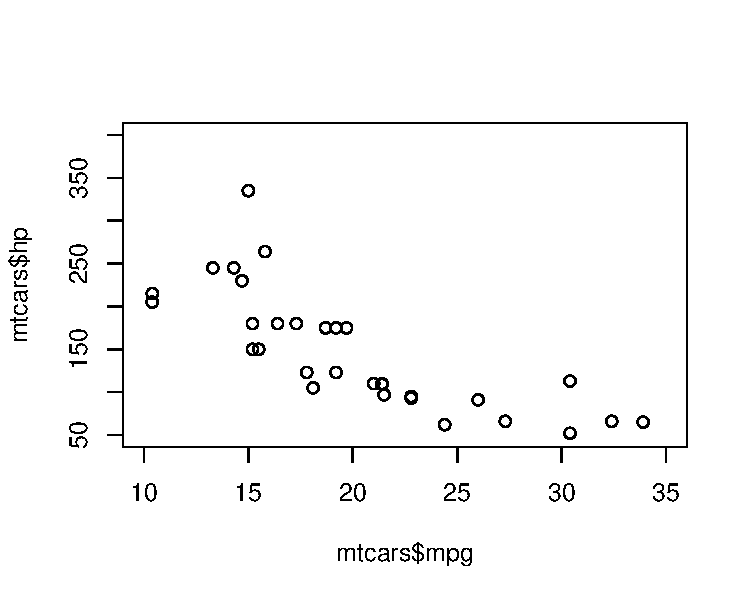
\includegraphics[width=.65\linewidth,height=.6\linewidth]{figure/unnamed-chunk-5-1} 

}



\end{knitrout}
\end{frame}

%------------------------------------------------

\begin{frame}[fragile]
\frametitle{Type}
\begin{knitrout}\footnotesize
\definecolor{shadecolor}{rgb}{0.969, 0.969, 0.969}\color{fgcolor}\begin{kframe}
\begin{alltt}
\hlcom{# using 'type' (e.g. lines)}
\hlkwd{plot}\hlstd{(mtcars}\hlopt{$}\hlstd{mpg, mtcars}\hlopt{$}\hlstd{hp,} \hlkwc{type} \hlstd{=} \hlstr{"l"}\hlstd{)}
\end{alltt}
\end{kframe}

{\centering 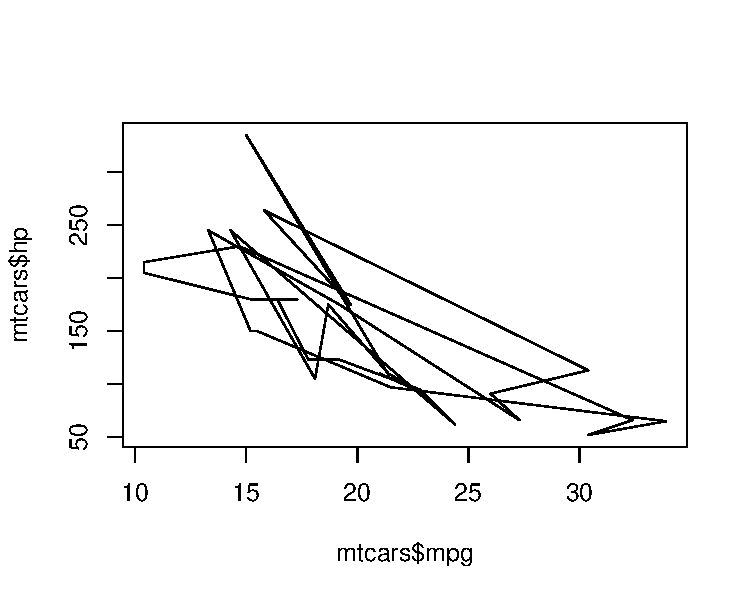
\includegraphics[width=.65\linewidth,height=.55\linewidth]{figure/unnamed-chunk-6-1} 

}



\end{knitrout}
\end{frame}

%------------------------------------------------

\begin{frame}[fragile]
\frametitle{Points}
\begin{knitrout}\footnotesize
\definecolor{shadecolor}{rgb}{0.969, 0.969, 0.969}\color{fgcolor}\begin{kframe}
\begin{alltt}
\hlcom{# character expansion 'cex'}
\hlcom{# and 'point character'}
\hlkwd{plot}\hlstd{(mtcars}\hlopt{$}\hlstd{mpg, mtcars}\hlopt{$}\hlstd{hp,} \hlkwc{cex} \hlstd{=} \hlnum{1.5}\hlstd{,} \hlkwc{pch} \hlstd{=} \hlnum{1}\hlstd{)}
\end{alltt}
\end{kframe}

{\centering 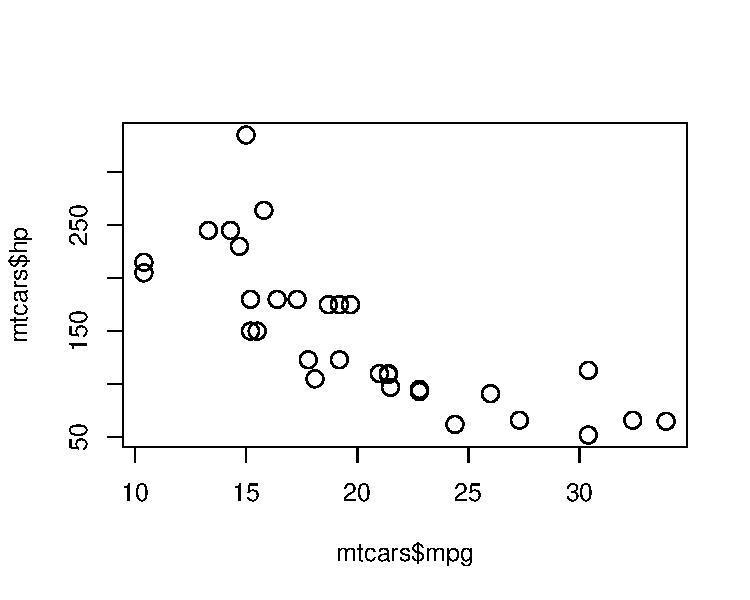
\includegraphics[width=.65\linewidth,height=.55\linewidth]{figure/unnamed-chunk-7-1} 

}



\end{knitrout}
\end{frame}

%------------------------------------------------

\begin{frame}[fragile]
\frametitle{Point symbols (\code{pch}) available in R}
\begin{knitrout}\scriptsize
\definecolor{shadecolor}{rgb}{0.969, 0.969, 0.969}\color{fgcolor}

{\centering 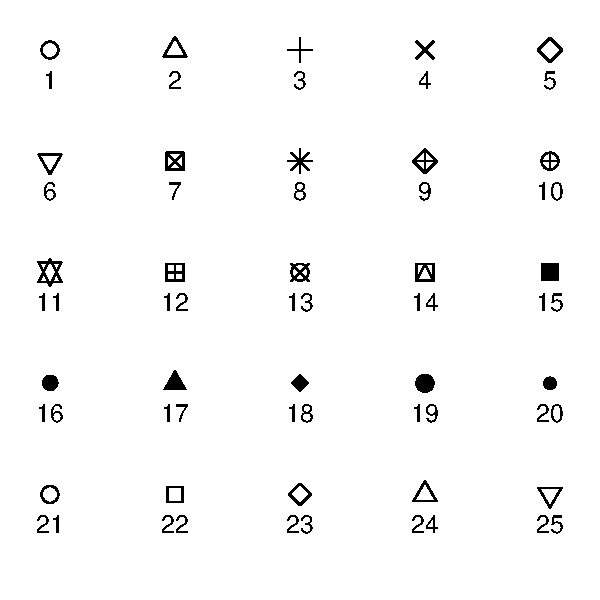
\includegraphics[width=.6\linewidth,height=.6\linewidth]{figure/points_pch-1} 

}



\end{knitrout}
\end{frame}

%------------------------------------------------

\begin{frame}[fragile]
\frametitle{Point Character}
\begin{knitrout}\scriptsize
\definecolor{shadecolor}{rgb}{0.969, 0.969, 0.969}\color{fgcolor}\begin{kframe}
\begin{alltt}
\hlcom{# 'pch' can be any character}
\hlkwd{plot}\hlstd{(mtcars}\hlopt{$}\hlstd{mpg, mtcars}\hlopt{$}\hlstd{hp,} \hlkwc{pch} \hlstd{=} \hlstr{"@"}\hlstd{)}
\end{alltt}
\end{kframe}

{\centering 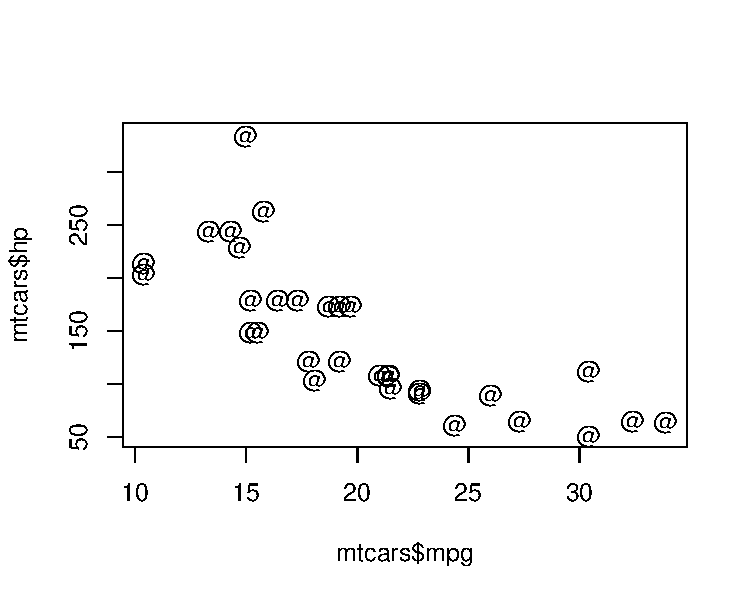
\includegraphics[width=.65\linewidth,height=.6\linewidth]{figure/unnamed-chunk-8-1} 

}



\end{knitrout}
\end{frame}

%------------------------------------------------

\begin{frame}[fragile]
\frametitle{Point Character}
\begin{knitrout}\scriptsize
\definecolor{shadecolor}{rgb}{0.969, 0.969, 0.969}\color{fgcolor}\begin{kframe}
\begin{alltt}
\hlcom{# 'pch' symbols will be recycled}
\hlkwd{plot}\hlstd{(mtcars}\hlopt{$}\hlstd{mpg, mtcars}\hlopt{$}\hlstd{hp,} \hlkwc{pch} \hlstd{=} \hlnum{1}\hlopt{:}\hlnum{25}\hlstd{)}
\end{alltt}
\end{kframe}

{\centering 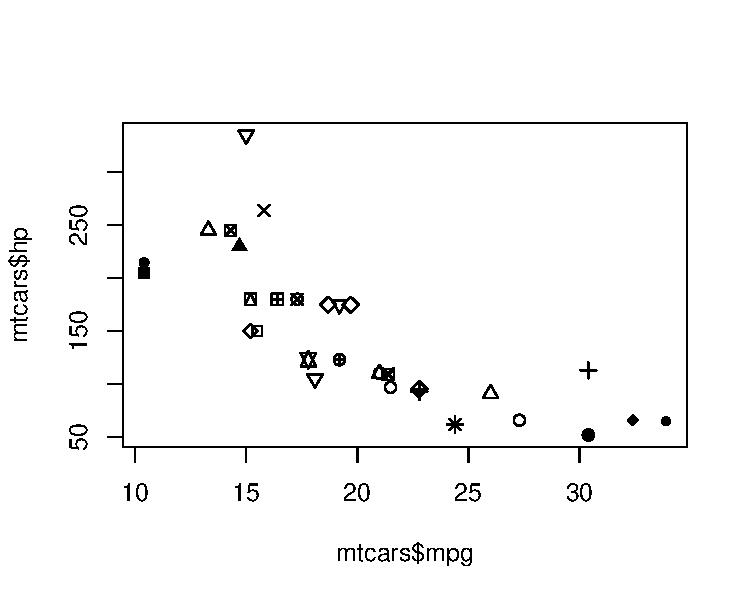
\includegraphics[width=.65\linewidth,height=.6\linewidth]{figure/unnamed-chunk-9-1} 

}



\end{knitrout}
\end{frame}

%------------------------------------------------

\begin{frame}[fragile]
\frametitle{Point Colors}
\begin{knitrout}\scriptsize
\definecolor{shadecolor}{rgb}{0.969, 0.969, 0.969}\color{fgcolor}\begin{kframe}
\begin{alltt}
\hlcom{# color argument 'col'}
\hlkwd{plot}\hlstd{(mtcars}\hlopt{$}\hlstd{mpg, mtcars}\hlopt{$}\hlstd{hp,} \hlkwc{pch} \hlstd{=} \hlnum{19}\hlstd{,} \hlkwc{col} \hlstd{=} \hlstr{"blue"}\hlstd{,} \hlkwc{cex} \hlstd{=} \hlnum{1.2}\hlstd{)}
\end{alltt}
\end{kframe}

{\centering 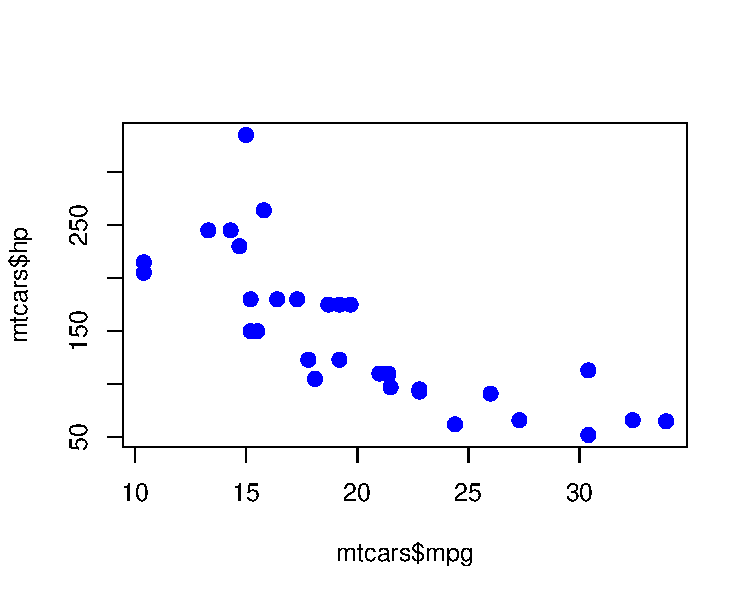
\includegraphics[width=.65\linewidth,height=.6\linewidth]{figure/unnamed-chunk-10-1} 

}



\end{knitrout}
\end{frame}

%------------------------------------------------

\begin{frame}[fragile]
\frametitle{Coloring Point Symbols}

\bi
  \item the \code{col} argument can be used to color symbols
  \item symbols 21 through 25 can additionally have
their interiors filled by using the \code{bg} (background) argument
\ei

\end{frame}

%------------------------------------------------

\begin{frame}[fragile]
\frametitle{Coloring Point symbols}
\begin{knitrout}\scriptsize
\definecolor{shadecolor}{rgb}{0.969, 0.969, 0.969}\color{fgcolor}

{\centering 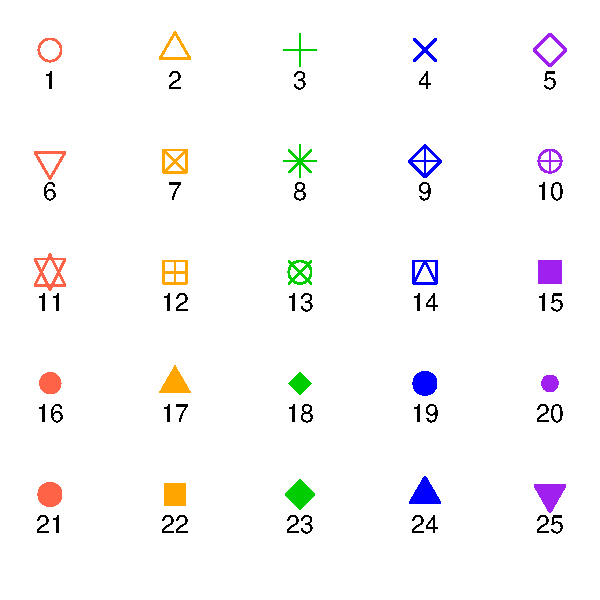
\includegraphics[width=.6\linewidth,height=.6\linewidth]{figure/points_cols-1} 

}



\end{knitrout}
\end{frame}

%------------------------------------------------

\begin{frame}[fragile]
\frametitle{So far ...}
\begin{knitrout}\footnotesize
\definecolor{shadecolor}{rgb}{0.969, 0.969, 0.969}\color{fgcolor}\begin{kframe}
\begin{alltt}
\hlcom{# using plot()}
\hlkwd{plot}\hlstd{(mtcars}\hlopt{$}\hlstd{mpg, mtcars}\hlopt{$}\hlstd{hp,}
     \hlkwc{xlim} \hlstd{=} \hlkwd{c}\hlstd{(}\hlnum{10}\hlstd{,} \hlnum{35}\hlstd{),} \hlkwc{ylim} \hlstd{=} \hlkwd{c}\hlstd{(}\hlnum{50}\hlstd{,} \hlnum{400}\hlstd{),}
     \hlkwc{xlab} \hlstd{=} \hlstr{"miles per gallon"}\hlstd{,}
     \hlkwc{ylab} \hlstd{=} \hlstr{"horsepower"}\hlstd{,}
     \hlkwc{main} \hlstd{=} \hlstr{"Simple Scatterplot"}\hlstd{,}
     \hlkwc{sub} \hlstd{=} \hlstr{'data matcars'}\hlstd{,}
     \hlkwc{pch} \hlstd{=} \hlnum{1}\hlopt{:}\hlnum{25}\hlstd{,} \hlkwc{cex} \hlstd{=} \hlnum{1.2}\hlstd{,} \hlkwc{col} \hlstd{=} \hlstr{"blue"}\hlstd{)}
\end{alltt}
\end{kframe}
\end{knitrout}
\end{frame}

%------------------------------------------------

\begin{frame}[fragile]
%\frametitle{So far ...}
\begin{knitrout}\footnotesize
\definecolor{shadecolor}{rgb}{0.969, 0.969, 0.969}\color{fgcolor}

{\centering 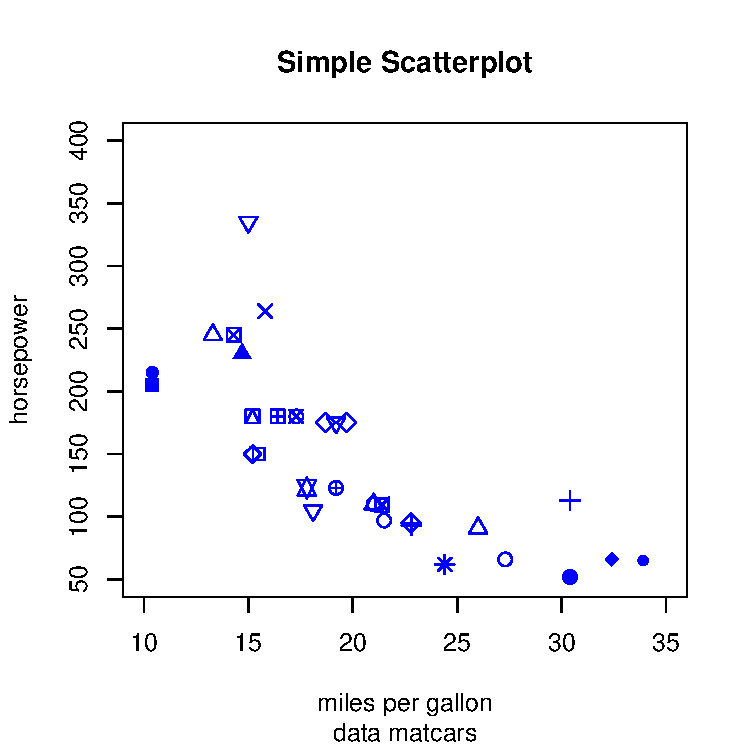
\includegraphics[width=.8\linewidth,height=.8\linewidth]{figure/plot_mtcars-1} 

}



\end{knitrout}
\end{frame}

%------------------------------------------------

\begin{frame}
\begin{center}
\Huge{\hilit{Low-Level Functions}}
\end{center}
\end{frame}

%------------------------------------------------

\begin{frame}
\frametitle{High and Low level functions}

\bi
  \item Usually we call a high-level function
  \item Most times we change the default arguments
  \item Then we call low-level functions
\ei

\end{frame}

%------------------------------------------------

\begin{frame}[fragile]
\frametitle{Scatter plot}
\begin{knitrout}\footnotesize
\definecolor{shadecolor}{rgb}{0.969, 0.969, 0.969}\color{fgcolor}\begin{kframe}
\begin{alltt}
\hlcom{# simple scatter-plot}
\hlkwd{plot}\hlstd{(mtcars}\hlopt{$}\hlstd{mpg, mtcars}\hlopt{$}\hlstd{hp)}

\hlcom{# adding text}
\hlkwd{text}\hlstd{(mtcars}\hlopt{$}\hlstd{mpg, mtcars}\hlopt{$}\hlstd{hp,} \hlkwc{labels} \hlstd{=} \hlkwd{rownames}\hlstd{(mtcars))}

\hlcom{# dummy legend}
\hlkwd{legend}\hlstd{(}\hlstr{"topright"}\hlstd{,} \hlkwc{legend} \hlstd{=} \hlstr{"a legend"}\hlstd{)}

\hlcom{# graphic title}
\hlkwd{title}\hlstd{(}\hlstr{"Miles Per Galon -vs- Horsepower"}\hlstd{)}
\end{alltt}
\end{kframe}
\end{knitrout}
\end{frame}

%------------------------------------------------

\begin{frame}[fragile]
\begin{knitrout}\footnotesize
\definecolor{shadecolor}{rgb}{0.969, 0.969, 0.969}\color{fgcolor}

{\centering 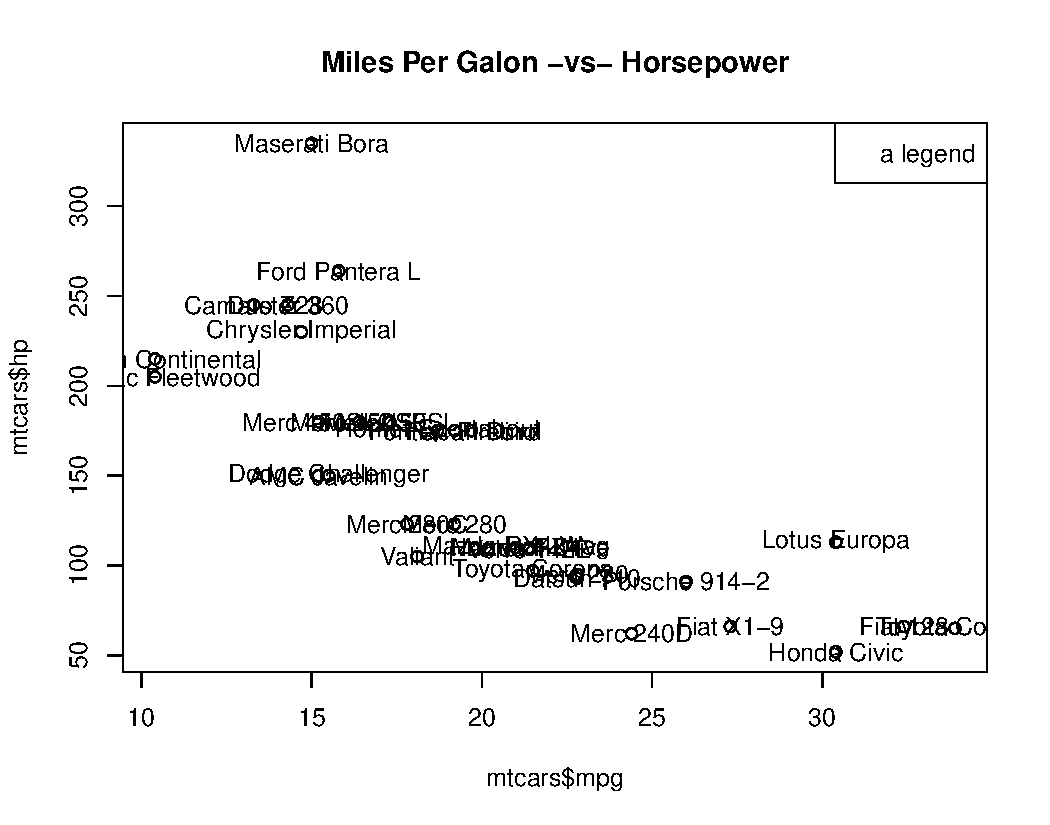
\includegraphics[width=.8\linewidth,height=.7\linewidth]{figure/mtcars_plot1-1} 

}



\end{knitrout}
\end{frame}

%------------------------------------------------

\begin{frame}[fragile]
\frametitle{Scatter plot}
\begin{knitrout}\footnotesize
\definecolor{shadecolor}{rgb}{0.969, 0.969, 0.969}\color{fgcolor}\begin{kframe}
\begin{alltt}
\hlcom{# simple scatter-plot}
\hlkwd{plot}\hlstd{(mtcars}\hlopt{$}\hlstd{mpg, mtcars}\hlopt{$}\hlstd{hp,} \hlkwc{type} \hlstd{=} \hlstr{"n"}\hlstd{,}
     \hlkwc{xlab} \hlstd{=} \hlstr{"miles per gallon"}\hlstd{,} \hlkwc{ylab} \hlstd{=} \hlstr{"horsepower"}\hlstd{)}
\hlcom{# grid lines}
\hlkwd{abline}\hlstd{(}\hlkwc{v} \hlstd{=} \hlkwd{seq}\hlstd{(}\hlkwc{from} \hlstd{=} \hlnum{10}\hlstd{,} \hlkwc{to} \hlstd{=} \hlnum{30}\hlstd{,} \hlkwc{by} \hlstd{=} \hlnum{5}\hlstd{),} \hlkwc{col} \hlstd{=} \hlstr{'gray'}\hlstd{)}
\hlkwd{abline}\hlstd{(}\hlkwc{h} \hlstd{=} \hlkwd{seq}\hlstd{(}\hlkwc{from} \hlstd{=} \hlnum{50}\hlstd{,} \hlkwc{to} \hlstd{=} \hlnum{300}\hlstd{,} \hlkwc{by} \hlstd{=} \hlnum{50}\hlstd{),} \hlkwc{col} \hlstd{=} \hlstr{' gray'}\hlstd{)}
\hlcom{# plot points}
\hlkwd{points}\hlstd{(mtcars}\hlopt{$}\hlstd{mpg, mtcars}\hlopt{$}\hlstd{hp,} \hlkwc{pch} \hlstd{=} \hlnum{19}\hlstd{,} \hlkwc{col} \hlstd{=} \hlstr{"blue"}\hlstd{)}
\hlcom{# plot text}
\hlkwd{text}\hlstd{(mtcars}\hlopt{$}\hlstd{mpg, mtcars}\hlopt{$}\hlstd{hp,} \hlkwc{labels} \hlstd{=} \hlkwd{rownames}\hlstd{(mtcars),}
     \hlkwc{pos} \hlstd{=} \hlnum{4}\hlstd{,} \hlkwc{col} \hlstd{=} \hlstr{"gray50"}\hlstd{)}
\hlcom{# graphic title}
\hlkwd{title}\hlstd{(}\hlstr{"Miles Per Galon -vs- Horsepower"}\hlstd{)}
\end{alltt}
\end{kframe}
\end{knitrout}
\end{frame}

%------------------------------------------------

\begin{frame}[fragile]
\begin{knitrout}\footnotesize
\definecolor{shadecolor}{rgb}{0.969, 0.969, 0.969}\color{fgcolor}

{\centering 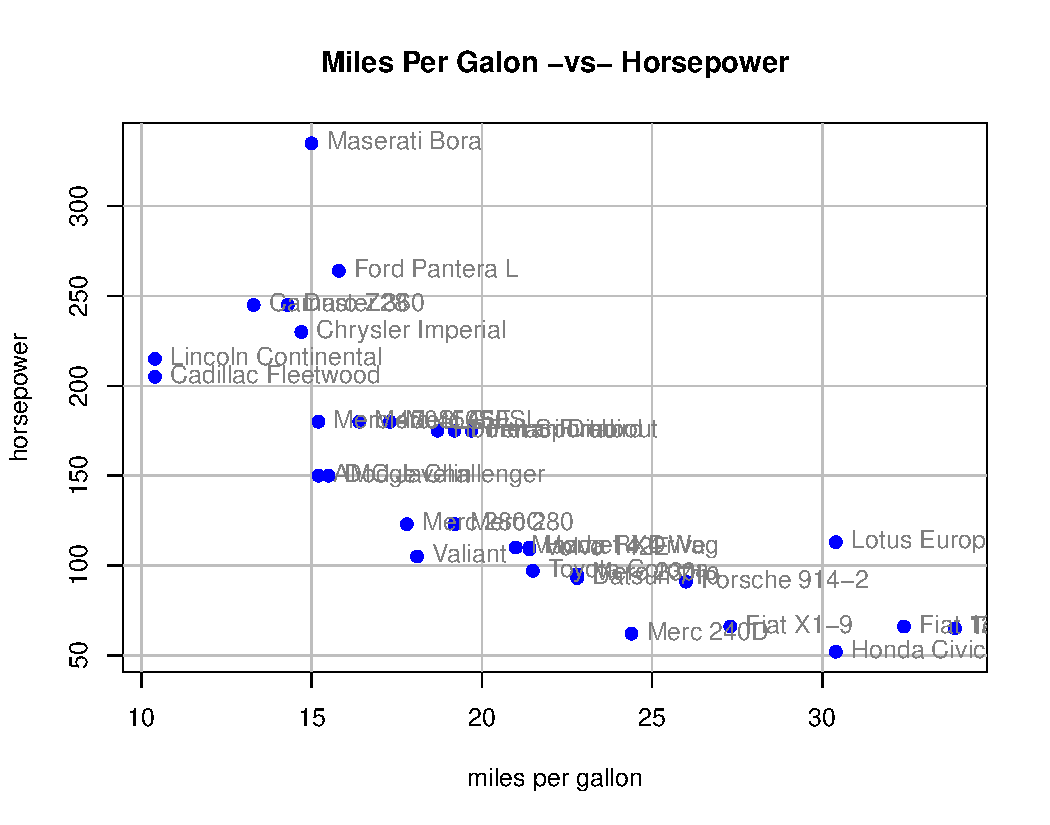
\includegraphics[width=.8\linewidth,height=.7\linewidth]{figure/mtcars_plot2-1} 

}



\end{knitrout}
\end{frame}

%------------------------------------------------

\begin{frame}
\frametitle{Test your knowledge}

\bb{The function \code{plot()}}
\bbi
  \item[A)] accepts any type of vector
  \item[B)] is a generic function
  \item[C)] works only for 1-D and 2-D objects
  \item[D)] is designed to display scatterplots and boxplots
\ei
\eb

\end{frame}

%------------------------------------------------

\begin{frame}
\frametitle{Low-level functions}

\begin{center}
 \begin{tabular}{l l}
  \hline
   Function & Description \\
  \hline
  \code{points()} & points \\  
  \code{lines()} & connected line segments \\
  \code{abline()} & straight lines across a plot \\
  \code{segments()} & disconnected line segments \\
  \code{arrows()} & arrows \\
  \code{rect()} & rectangles \\
  \code{polygon()} & polygons \\
  \code{text()} & text \\
  \code{symbols()} & various symbols \\
  \code{legend()} & legends \\
  \hline
 \end{tabular}
\end{center}

\end{frame}

%------------------------------------------------

\begin{frame}[fragile]
\frametitle{Drawing Points with \code{points()}}

\begin{verbatim}
points(x, y, pch = int, col = str)
\end{verbatim}

\bi
  \item \code{pch} integer or string indicating type of point character
  \item \code{col} color of points
\ei

\end{frame}

%------------------------------------------------

\begin{frame}[fragile]
\begin{knitrout}\scriptsize
\definecolor{shadecolor}{rgb}{0.969, 0.969, 0.969}\color{fgcolor}\begin{kframe}
\begin{alltt}
\hlcom{# drawing points}
\hlkwd{plot}\hlstd{(mtcars}\hlopt{$}\hlstd{mpg, mtcars}\hlopt{$}\hlstd{hp,} \hlkwc{type} \hlstd{=} \hlstr{"n"}\hlstd{)}
\hlkwd{points}\hlstd{(mtcars}\hlopt{$}\hlstd{mpg, mtcars}\hlopt{$}\hlstd{hp)}
\end{alltt}
\end{kframe}

{\centering 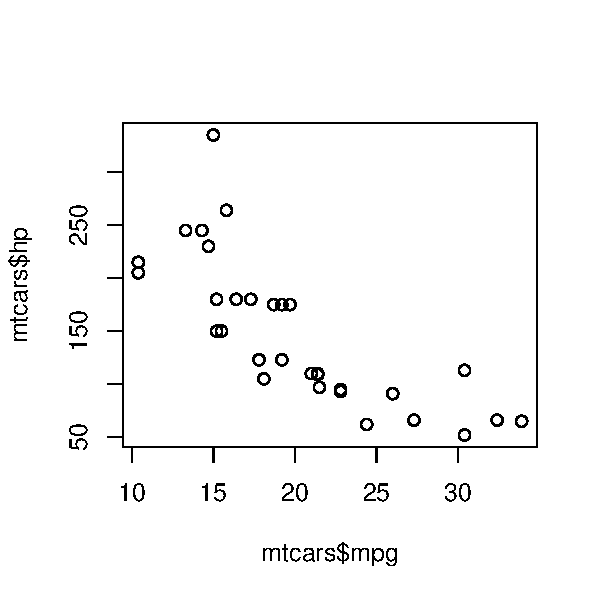
\includegraphics[width=.6\linewidth,height=.6\linewidth]{figure/unnamed-chunk-11-1} 

}



\end{knitrout}
\end{frame}

%------------------------------------------------

\begin{frame}[fragile]
\frametitle{Connected Line Segments}

\begin{verbatim}
lines(x, y, lty = str, lwd = num, col = str)
\end{verbatim}
\bi
  \item \code{lty} specifies the line texture. It should be one of \code{"blank"} (0), \code{"solid"} (1), \code{"dashed"}(2), \code{"dotted"} (3), \code{"dotdash"} (4), \code{"longdash"} (5) or \code{"twodash"} (6).
  \item \code{lwd} and \code{col} specify the line width and colour
\ei

\end{frame}

%------------------------------------------------

\begin{frame}[fragile]
\begin{knitrout}\scriptsize
\definecolor{shadecolor}{rgb}{0.969, 0.969, 0.969}\color{fgcolor}\begin{kframe}
\begin{alltt}
\hlcom{# connected lines}
\hlkwd{plot}\hlstd{(mtcars}\hlopt{$}\hlstd{mpg, mtcars}\hlopt{$}\hlstd{hp,} \hlkwc{type} \hlstd{=} \hlstr{"n"}\hlstd{)}
\hlkwd{lines}\hlstd{(mtcars}\hlopt{$}\hlstd{mpg, mtcars}\hlopt{$}\hlstd{hp,} \hlkwc{type} \hlstd{=} \hlstr{"s"}\hlstd{,} \hlkwc{lwd} \hlstd{=} \hlnum{2}\hlstd{)}
\end{alltt}
\end{kframe}

{\centering 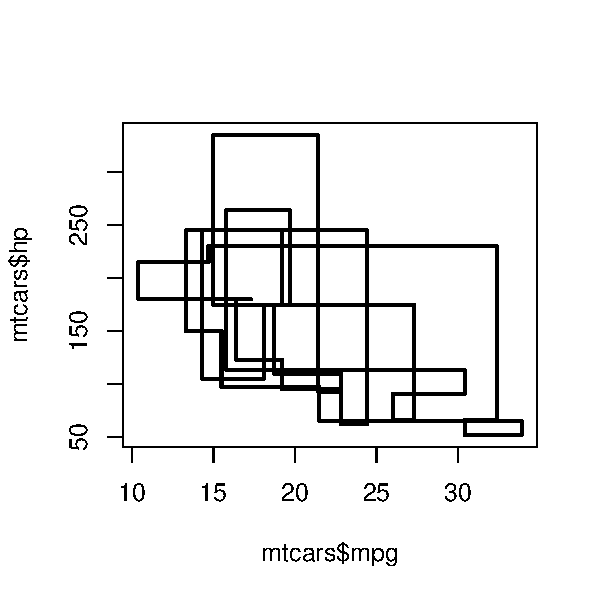
\includegraphics[width=.6\linewidth,height=.6\linewidth]{figure/unnamed-chunk-12-1} 

}



\end{knitrout}
\end{frame}

%------------------------------------------------

\begin{frame}
\frametitle{Line Graph Options}

The \code{type} argument can be used to produced other types of lines
\bi
  \item \code{type = "l"} line graph
  \item \code{type = "s"} step function (horizontal first)
  \item \code{type = "S"} step function (vertical first)
  \item \code{type = "h"} high density (needle) plot
  \item \code{type = "p"} draw points
  \item \code{type = "b"} draw points and lines
  \item \code{type = "o"} over-plotting points and lines
\ei

\end{frame}

%------------------------------------------------

\begin{frame}[fragile]
\frametitle{Line Graph Options}
\begin{knitrout}\scriptsize
\definecolor{shadecolor}{rgb}{0.969, 0.969, 0.969}\color{fgcolor}

{\centering 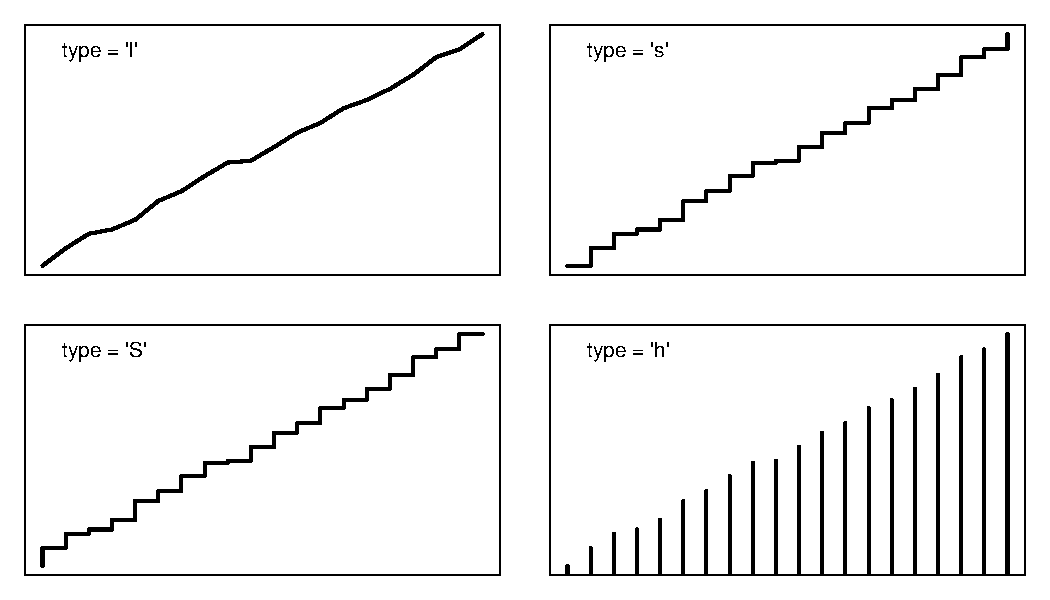
\includegraphics[width=.9\linewidth,height=.6\linewidth]{figure/line_types-1} 

}



\end{knitrout}
\end{frame}

%------------------------------------------------

\begin{frame}[fragile]
\frametitle{Connected Line Segments}
\begin{knitrout}\footnotesize
\definecolor{shadecolor}{rgb}{0.969, 0.969, 0.969}\color{fgcolor}\begin{kframe}
\begin{alltt}
\hlstd{x} \hlkwb{<-} \hlnum{2005}\hlopt{:}\hlnum{2015}
\hlstd{y} \hlkwb{<-} \hlkwd{c}\hlstd{(}\hlnum{81}\hlstd{,} \hlnum{83}\hlstd{,} \hlnum{84.3}\hlstd{,} \hlnum{85}\hlstd{,} \hlnum{85.4}\hlstd{,} \hlnum{86.5}\hlstd{,} \hlnum{88.3}\hlstd{,}
       \hlnum{88.6}\hlstd{,} \hlnum{90.8}\hlstd{,} \hlnum{91.1}\hlstd{,} \hlnum{91.3}\hlstd{)}

\hlkwd{plot}\hlstd{(x, y,} \hlkwc{type} \hlstd{=} \hlstr{'n'}\hlstd{,} \hlkwc{xlab} \hlstd{=} \hlstr{"Time"}\hlstd{,} \hlkwc{ylab} \hlstd{=} \hlstr{"Values"}\hlstd{)}
\hlkwd{lines}\hlstd{(x, y,} \hlkwc{lwd} \hlstd{=} \hlnum{2}\hlstd{)}
\hlkwd{title}\hlstd{(}\hlkwc{main} \hlstd{=} \hlstr{"Line Graph Example"}\hlstd{)}
\end{alltt}
\end{kframe}
\end{knitrout}
\end{frame}

%------------------------------------------------

\begin{frame}[fragile]
\frametitle{Connected Line Segments}
\begin{knitrout}\scriptsize
\definecolor{shadecolor}{rgb}{0.969, 0.969, 0.969}\color{fgcolor}

{\centering 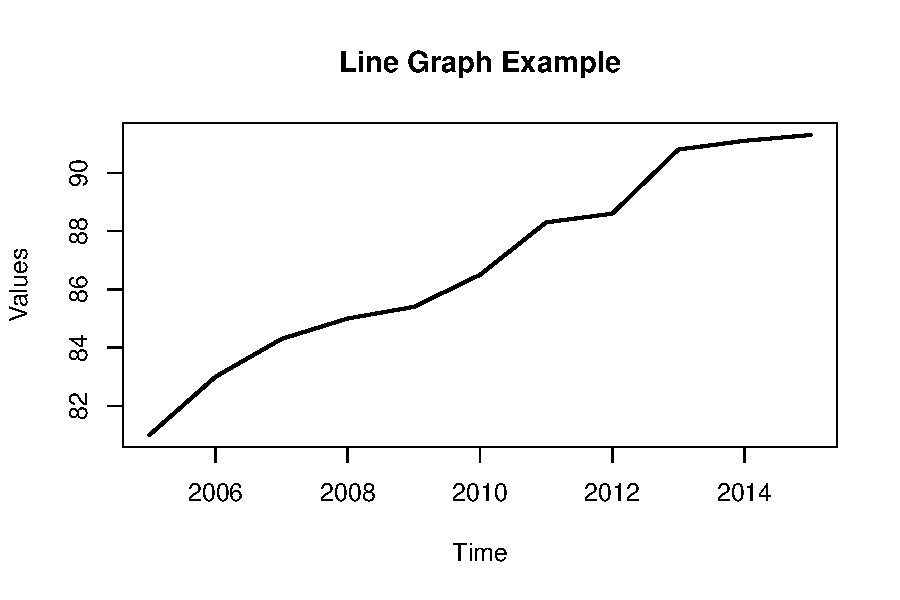
\includegraphics[width=.8\linewidth,height=.6\linewidth]{figure/line_segs-1} 

}



\end{knitrout}
\end{frame}

%------------------------------------------------

\begin{frame}[fragile]
\frametitle{Drawing Straight Lines}

\begin{verbatim}
abline(a = intercept, b = slope)
abline(h = numbers)
abline(v = numbers)
\end{verbatim}

\bi
  \item The \code{a / b} form specifies a line in intercept / slope form
  \item \code{h} specifies horizontal lines at given y-values
  \item \code{v} specifies vartical lines at given x-values
\ei

\end{frame}

%------------------------------------------------

\begin{frame}[fragile]
\begin{knitrout}\scriptsize
\definecolor{shadecolor}{rgb}{0.969, 0.969, 0.969}\color{fgcolor}\begin{kframe}
\begin{alltt}
\hlcom{# drawing straight lines}
\hlkwd{plot}\hlstd{(mtcars}\hlopt{$}\hlstd{mpg, mtcars}\hlopt{$}\hlstd{hp,} \hlkwc{type} \hlstd{=} \hlstr{"n"}\hlstd{)}
\hlkwd{abline}\hlstd{(}\hlkwc{v} \hlstd{=} \hlkwd{seq}\hlstd{(}\hlnum{10}\hlstd{,} \hlnum{30}\hlstd{,} \hlkwc{by} \hlstd{=} \hlnum{5}\hlstd{),} \hlkwc{h} \hlstd{=} \hlkwd{seq}\hlstd{(}\hlnum{50}\hlstd{,} \hlnum{300}\hlstd{,} \hlkwc{by} \hlstd{=} \hlnum{50}\hlstd{))}
\hlkwd{points}\hlstd{(mtcars}\hlopt{$}\hlstd{mpg, mtcars}\hlopt{$}\hlstd{hp,} \hlkwc{pch} \hlstd{=} \hlnum{19}\hlstd{,} \hlkwc{col} \hlstd{=} \hlstr{"red"}\hlstd{)}
\end{alltt}
\end{kframe}

{\centering 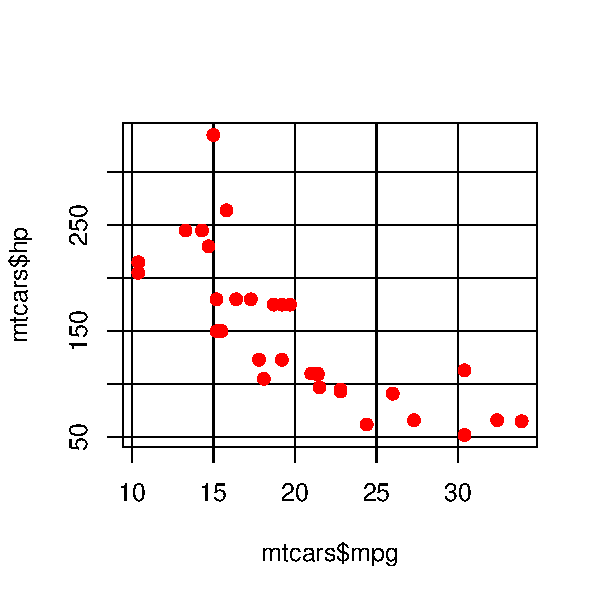
\includegraphics[width=.6\linewidth,height=.6\linewidth]{figure/unnamed-chunk-13-1} 

}



\end{knitrout}
\end{frame}

%------------------------------------------------

\begin{frame}[fragile]
\frametitle{Drawing Disconnected Lines}

Disconnected lines can be drawn with the function:
\begin{verbatim}
segments(x0, y0, x1, y1)
\end{verbatim}

\bi
  \item The \code{x0, y0, x1, y1} arguments give the start and end coordinates of the segments.
  \item Line texture, colour and width arguments can also be
given.
\ei

\end{frame}

%------------------------------------------------

\begin{frame}[fragile]
\frametitle{Drawing Line Segments}
\begin{knitrout}\footnotesize
\definecolor{shadecolor}{rgb}{0.969, 0.969, 0.969}\color{fgcolor}\begin{kframe}
\begin{alltt}
\hlstd{n} \hlkwb{<-} \hlnum{11}
\hlstd{theta} \hlkwb{<-} \hlkwd{seq}\hlstd{(}\hlnum{0}\hlstd{,} \hlnum{2} \hlopt{*} \hlstd{pi,} \hlkwc{length} \hlstd{= n} \hlopt{+} \hlnum{1}\hlstd{)[}\hlnum{1}\hlopt{:}\hlstd{n]}
\hlstd{x} \hlkwb{<-} \hlkwd{sin}\hlstd{(theta)}
\hlstd{y} \hlkwb{<-} \hlkwd{cos}\hlstd{(theta)}
\hlstd{v1} \hlkwb{<-} \hlkwd{rep}\hlstd{(}\hlnum{1}\hlopt{:}\hlstd{n, n)}
\hlstd{v2} \hlkwb{<-} \hlkwd{rep}\hlstd{(}\hlnum{1}\hlopt{:}\hlstd{n,} \hlkwd{rep}\hlstd{(n, n))}

\hlkwd{plot}\hlstd{(x, y,} \hlkwc{type} \hlstd{=} \hlstr{'n'}\hlstd{)}
\hlkwd{segments}\hlstd{(x[v1], y[v1], x[v2], y[v2])}
\end{alltt}
\end{kframe}
\end{knitrout}
\end{frame}

%------------------------------------------------

\begin{frame}[fragile]
\begin{knitrout}\scriptsize
\definecolor{shadecolor}{rgb}{0.969, 0.969, 0.969}\color{fgcolor}

{\centering 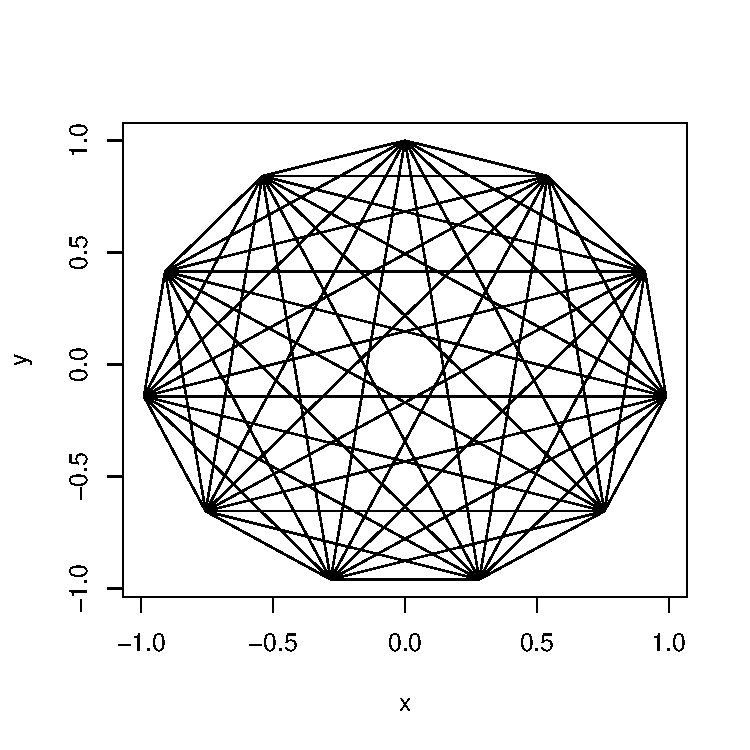
\includegraphics[width=.8\linewidth,height=.8\linewidth]{figure/segments-1} 

}



\end{knitrout}
\end{frame}

%------------------------------------------------

\begin{frame}[fragile]
\frametitle{Drawing Polygons}

Polygons can be drawn with the function:
\begin{verbatim}
polygon(x, y, col = str, border = str)
\end{verbatim}

\bi
  \item \code{x, y} give the coordinates of the polygon vertexes. \code{NA} values separate polygons.
  \item \code{col} specifies the color of the interior.
  \item \code{border} specifies the color of the border.
  \item line texture and width specifications can also be given
\ei

\end{frame}

%------------------------------------------------

\begin{frame}[fragile]
\frametitle{Drawing Polygons}
\begin{knitrout}\scriptsize
\definecolor{shadecolor}{rgb}{0.969, 0.969, 0.969}\color{fgcolor}

{\centering 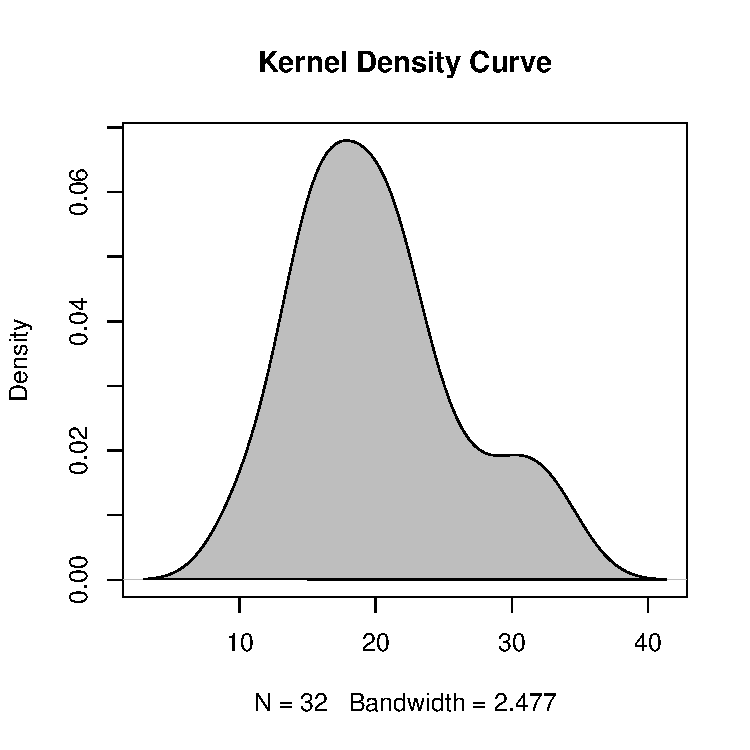
\includegraphics[width=.6\linewidth,height=.6\linewidth]{figure/polygons-1} 

}



\end{knitrout}
\end{frame}

%------------------------------------------------

\begin{frame}[fragile]
\frametitle{Adding Text}

We can add text using the function:
\begin{verbatim}
text(x, y, labels, ...)
\end{verbatim}

\bi
  \item \code{x, y} give the coordinates of the text.
  \item \code{labels} gives the actual text strings.
  \item \code{font} optional font for the text.
  \item \code{col} optional color for the text.
  \item \code{srt} rotation of the text.
  \item \code{adj} justification of the text.
\ei

\end{frame}

%------------------------------------------------

\begin{frame}[fragile]
\frametitle{Drawing Text}
\begin{knitrout}\footnotesize
\definecolor{shadecolor}{rgb}{0.969, 0.969, 0.969}\color{fgcolor}\begin{kframe}
\begin{alltt}
\hlkwd{plot}\hlstd{(}\hlnum{0.5}\hlstd{,} \hlnum{0.5}\hlstd{,} \hlkwc{xlim} \hlstd{=} \hlkwd{c}\hlstd{(}\hlnum{0}\hlstd{,} \hlnum{1}\hlstd{),} \hlkwc{ylim} \hlstd{=} \hlkwd{c}\hlstd{(}\hlnum{0}\hlstd{,} \hlnum{1}\hlstd{),} \hlkwc{type} \hlstd{=} \hlstr{'n'}\hlstd{)}
\hlkwd{abline}\hlstd{(}\hlkwc{h} \hlstd{=} \hlkwd{c}\hlstd{(}\hlnum{.2}\hlstd{,} \hlnum{.5}\hlstd{,} \hlnum{.8}\hlstd{),}
       \hlkwc{v} \hlstd{=} \hlkwd{c}\hlstd{(}\hlnum{.5}\hlstd{,} \hlnum{.2}\hlstd{,} \hlnum{.8}\hlstd{),} \hlkwc{col} \hlstd{=} \hlstr{"lightgrey"}\hlstd{)}
\hlkwd{text}\hlstd{(}\hlnum{0.5}\hlstd{,} \hlnum{0.5}\hlstd{,} \hlstr{"srt = 45, adj = c(.5, .5)"}\hlstd{,}
     \hlkwc{srt} \hlstd{=} \hlnum{45}\hlstd{,} \hlkwc{adj} \hlstd{=} \hlkwd{c}\hlstd{(}\hlnum{.5}\hlstd{,} \hlnum{.5}\hlstd{))}
\hlkwd{text}\hlstd{(}\hlnum{0.5}\hlstd{,} \hlnum{0.8}\hlstd{,} \hlstr{"adj = c(0, .5)"}\hlstd{,} \hlkwc{adj} \hlstd{=} \hlkwd{c}\hlstd{(}\hlnum{0}\hlstd{,} \hlnum{.5}\hlstd{))}
\hlkwd{text}\hlstd{(}\hlnum{0.5}\hlstd{,} \hlnum{0.2}\hlstd{,} \hlstr{"adj = c(1, .5)"}\hlstd{,} \hlkwc{adj} \hlstd{=} \hlkwd{c}\hlstd{(}\hlnum{1}\hlstd{,} \hlnum{.5}\hlstd{))}
\hlkwd{text}\hlstd{(}\hlnum{0.2}\hlstd{,} \hlnum{0.5}\hlstd{,} \hlstr{"adj = c(1, 1)"}\hlstd{,} \hlkwc{adj} \hlstd{=} \hlkwd{c}\hlstd{(}\hlnum{1}\hlstd{,} \hlnum{1}\hlstd{))}
\hlkwd{text}\hlstd{(}\hlnum{0.8}\hlstd{,} \hlnum{0.5}\hlstd{,} \hlstr{"adj = c(0, 0)"}\hlstd{,} \hlkwc{adj} \hlstd{=} \hlkwd{c}\hlstd{(}\hlnum{0}\hlstd{,} \hlnum{0}\hlstd{))}
\end{alltt}
\end{kframe}
\end{knitrout}
\end{frame}

%------------------------------------------------

\begin{frame}[fragile]
\frametitle{Drawing Text}
\begin{knitrout}\scriptsize
\definecolor{shadecolor}{rgb}{0.969, 0.969, 0.969}\color{fgcolor}

{\centering 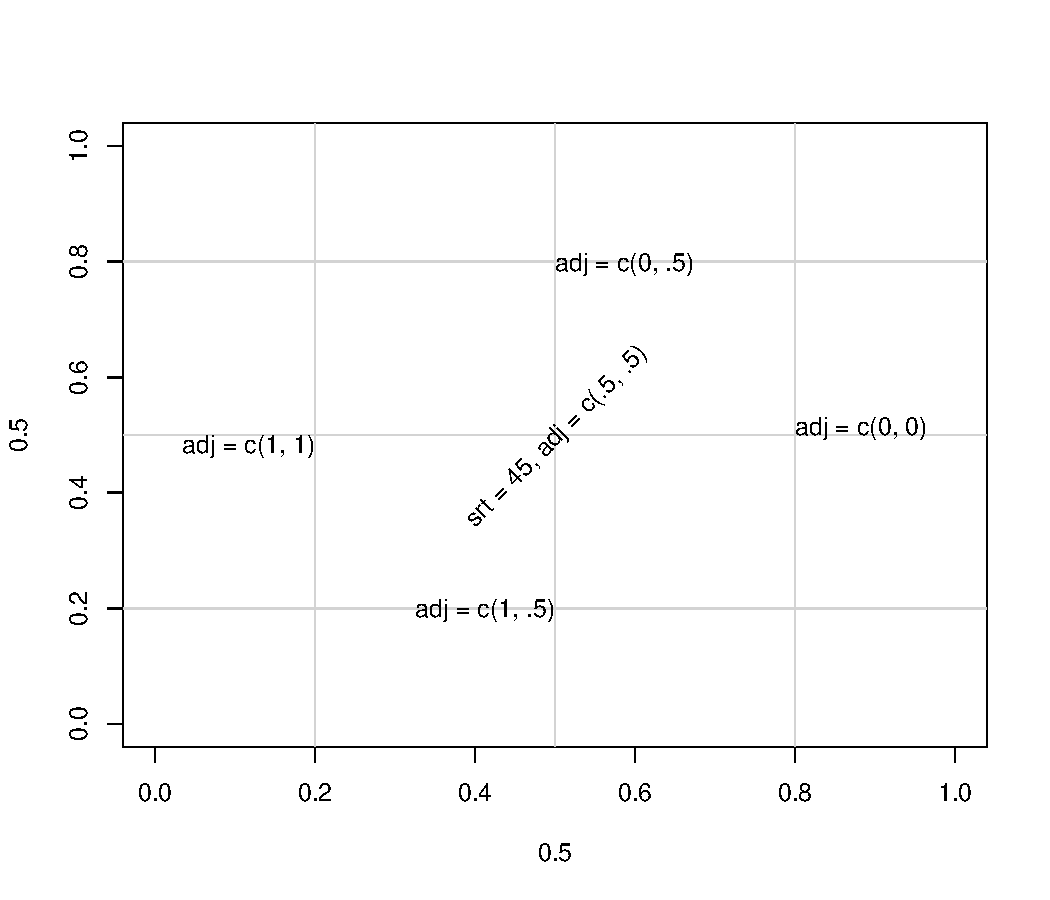
\includegraphics[width=.8\linewidth,height=.75\linewidth]{figure/draw_text-1} 

}



\end{knitrout}
\end{frame}

%------------------------------------------------

\begin{frame}[fragile]
\frametitle{Adding a Legend}

Legends can be added with:
\begin{verbatim}
legend(xloc, yloc, legend = text
       lty = linetypes, lwd = linewidths,
       pch = glyphname, col = colours,
       xjust = justification, yjust = justification)
\end{verbatim}

\bi
  \item \code{xloc} and \code{yloc} give the coordinates where the legend is to be placed
  \item \code{xjust} and \code{yjust} give
the justification of the legend box with respect to
the location. 
\ei

\end{frame}

%------------------------------------------------

\begin{frame}[fragile]
\frametitle{Adding Legends}
\begin{knitrout}\scriptsize
\definecolor{shadecolor}{rgb}{0.969, 0.969, 0.969}\color{fgcolor}\begin{kframe}
\begin{alltt}
\hlcom{# coords of exact line}
\hlkwd{plot}\hlstd{(mtcars}\hlopt{$}\hlstd{mpg, mtcars}\hlopt{$}\hlstd{hp)}
\hlkwd{legend}\hlstd{(}\hlstr{"topright"}\hlstd{,} \hlkwc{legend} \hlstd{=} \hlstr{"A legend"}\hlstd{)}
\end{alltt}
\end{kframe}

{\centering 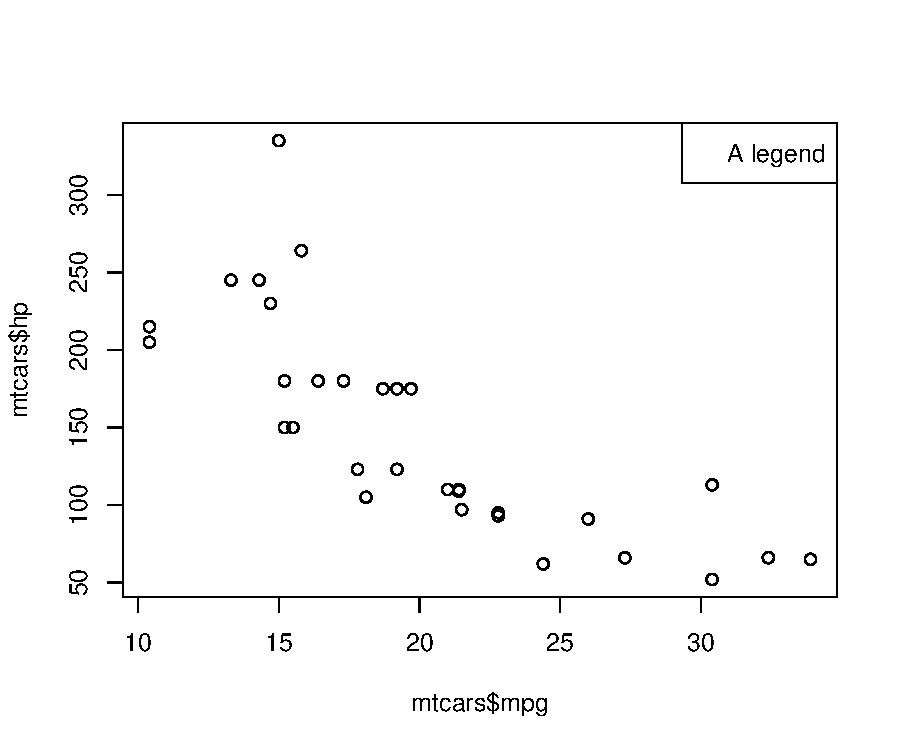
\includegraphics[width=.7\linewidth,height=.6\linewidth]{figure/add_legend-1} 

}



\end{knitrout}
\end{frame}

%------------------------------------------------

\begin{frame}
\begin{center}
\Huge{\hilit{Plots from scratch}}
\end{center}
\end{frame}

%------------------------------------------------

\begin{frame}
\frametitle{Customizing Annotations}

It is also possible to create a plot from scratch. Although this procedure is less documented, it is extremely flexible:
\begin{enumerate}
  \item call \code{plot.new()} to start a new plot frame
  \item call \code{plot.window()} to define coordinates
  \item then call low-level functions:
  \item typical options involve \code{axis()}
  \item then \code{title()} (title, subtitle)
  \item after that call other function: e.g. \code{points()}, \code{lines()}, etc
\end{enumerate}

\end{frame}

%------------------------------------------------

\begin{frame}[fragile]
\frametitle{Plot from Scratch}
\begin{knitrout}\footnotesize
\definecolor{shadecolor}{rgb}{0.969, 0.969, 0.969}\color{fgcolor}\begin{kframe}
\begin{alltt}
\hlkwd{plot.new}\hlstd{()}
\hlkwd{plot.window}\hlstd{(}\hlkwc{xlim} \hlstd{=} \hlkwd{c}\hlstd{(}\hlnum{0}\hlstd{,} \hlnum{10}\hlstd{),} \hlkwc{ylim} \hlstd{=} \hlkwd{c}\hlstd{(}\hlopt{-}\hlnum{2}\hlstd{,} \hlnum{4}\hlstd{),} \hlkwc{xaxs} \hlstd{=} \hlstr{"i"}\hlstd{)}
\hlkwd{axis}\hlstd{(}\hlnum{1}\hlstd{,} \hlkwc{col.axis} \hlstd{=} \hlstr{"grey30"}\hlstd{)}
\hlkwd{axis}\hlstd{(}\hlnum{2}\hlstd{,} \hlkwc{col.axis} \hlstd{=} \hlstr{"grey30"}\hlstd{,} \hlkwc{las} \hlstd{=} \hlnum{1}\hlstd{)}
\hlkwd{title}\hlstd{(}\hlkwc{main} \hlstd{=} \hlstr{"Main Title"}\hlstd{,}
      \hlkwc{col.main} \hlstd{=} \hlstr{"tomato"}\hlstd{,}
      \hlkwc{sub} \hlstd{=} \hlstr{"Plot Subtitle"}\hlstd{,}
      \hlkwc{col.sub} \hlstd{=} \hlstr{"orange"}\hlstd{,}
      \hlkwc{xlab} \hlstd{=} \hlstr{"x-axis"}\hlstd{,} \hlkwc{ylab} \hlstd{=} \hlstr{"y-axis"}\hlstd{,}
      \hlkwc{col.lab} \hlstd{=} \hlstr{"blue"}\hlstd{,} \hlkwc{font.lab} \hlstd{=} \hlnum{3}\hlstd{)}
\hlkwd{box}\hlstd{(}\hlstr{"figure"}\hlstd{,} \hlkwc{col} \hlstd{=} \hlstr{"grey90"}\hlstd{)}
\end{alltt}
\end{kframe}
\end{knitrout}
\end{frame}

%------------------------------------------------

\begin{frame}[fragile]
\frametitle{Plot from Scratch}
\begin{knitrout}\scriptsize
\definecolor{shadecolor}{rgb}{0.969, 0.969, 0.969}\color{fgcolor}

{\centering 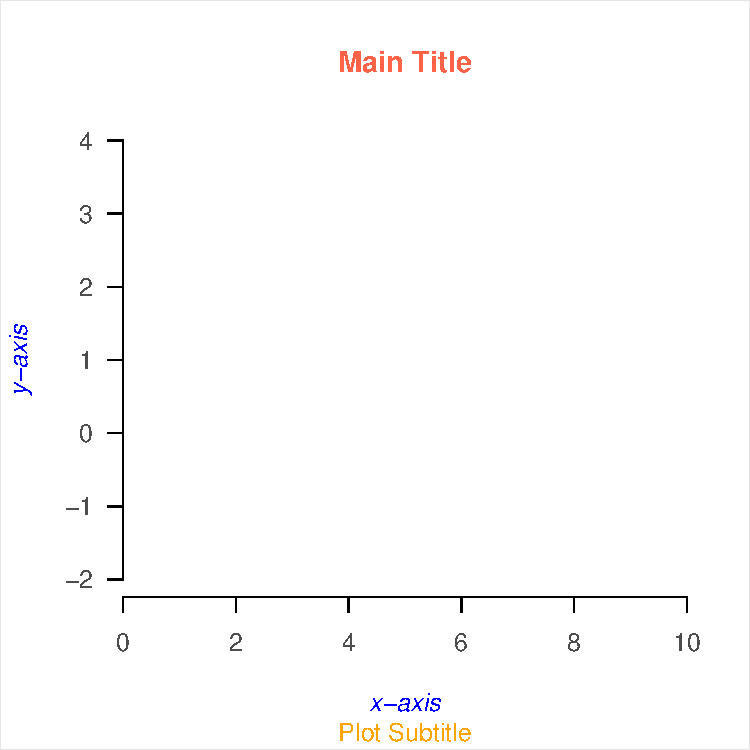
\includegraphics[width=.6\linewidth,height=.6\linewidth]{figure/bare_plot-1} 

}



\end{knitrout}
\end{frame}

%------------------------------------------------

\begin{frame}[fragile]
\frametitle{Another plot from scratch}
\begin{knitrout}\footnotesize
\definecolor{shadecolor}{rgb}{0.969, 0.969, 0.969}\color{fgcolor}\begin{kframe}
\begin{alltt}
\hlkwd{set.seed}\hlstd{(}\hlnum{5}\hlstd{)}
\hlstd{x} \hlkwb{<-} \hlkwd{rnorm}\hlstd{(}\hlnum{200}\hlstd{)}
\hlstd{y} \hlkwb{<-} \hlstd{x} \hlopt{+} \hlkwd{rnorm}\hlstd{(}\hlnum{200}\hlstd{)}

\hlkwd{plot.new}\hlstd{()}
\hlkwd{plot.window}\hlstd{(}\hlkwc{xlim} \hlstd{=} \hlkwd{c}\hlstd{(}\hlopt{-}\hlnum{4.5}\hlstd{,} \hlnum{4.5}\hlstd{),} \hlkwc{xaxs} \hlstd{=} \hlstr{"i"}\hlstd{,}
            \hlkwc{ylim} \hlstd{=} \hlkwd{c}\hlstd{(}\hlopt{-}\hlnum{4.5}\hlstd{,} \hlnum{4.5}\hlstd{),} \hlkwc{yaxs} \hlstd{=} \hlstr{"i"}\hlstd{)}
\hlstd{z} \hlkwb{<-} \hlkwd{lm}\hlstd{(y} \hlopt{~} \hlstd{x)}
\hlkwd{abline}\hlstd{(}\hlkwc{h} \hlstd{=} \hlopt{-}\hlnum{4}\hlopt{:}\hlnum{4}\hlstd{,} \hlkwc{v} \hlstd{=} \hlopt{-}\hlnum{4}\hlopt{:}\hlnum{4}\hlstd{,} \hlkwc{col} \hlstd{=} \hlstr{"lightgrey"}\hlstd{)}
\hlkwd{abline}\hlstd{(}\hlkwc{a} \hlstd{=} \hlkwd{coef}\hlstd{(z)[}\hlnum{1}\hlstd{],} \hlkwc{b} \hlstd{=} \hlkwd{coef}\hlstd{(z)[}\hlnum{2}\hlstd{],} \hlkwc{lwd} \hlstd{=} \hlnum{2}\hlstd{,} \hlkwc{col} \hlstd{=} \hlstr{"red"}\hlstd{)}
\hlkwd{points}\hlstd{(x, y)}
\hlkwd{axis}\hlstd{(}\hlnum{1}\hlstd{)}
\hlkwd{axis}\hlstd{(}\hlnum{2}\hlstd{,} \hlkwc{las} \hlstd{=} \hlnum{1}\hlstd{)}
\hlkwd{box}\hlstd{()}
\hlkwd{title}\hlstd{(}\hlkwc{main} \hlstd{=} \hlstr{"A Fitted Regression Line"}\hlstd{)}
\end{alltt}
\end{kframe}
\end{knitrout}
\end{frame}

%------------------------------------------------

\begin{frame}[fragile]
\begin{knitrout}\scriptsize
\definecolor{shadecolor}{rgb}{0.969, 0.969, 0.969}\color{fgcolor}

{\centering 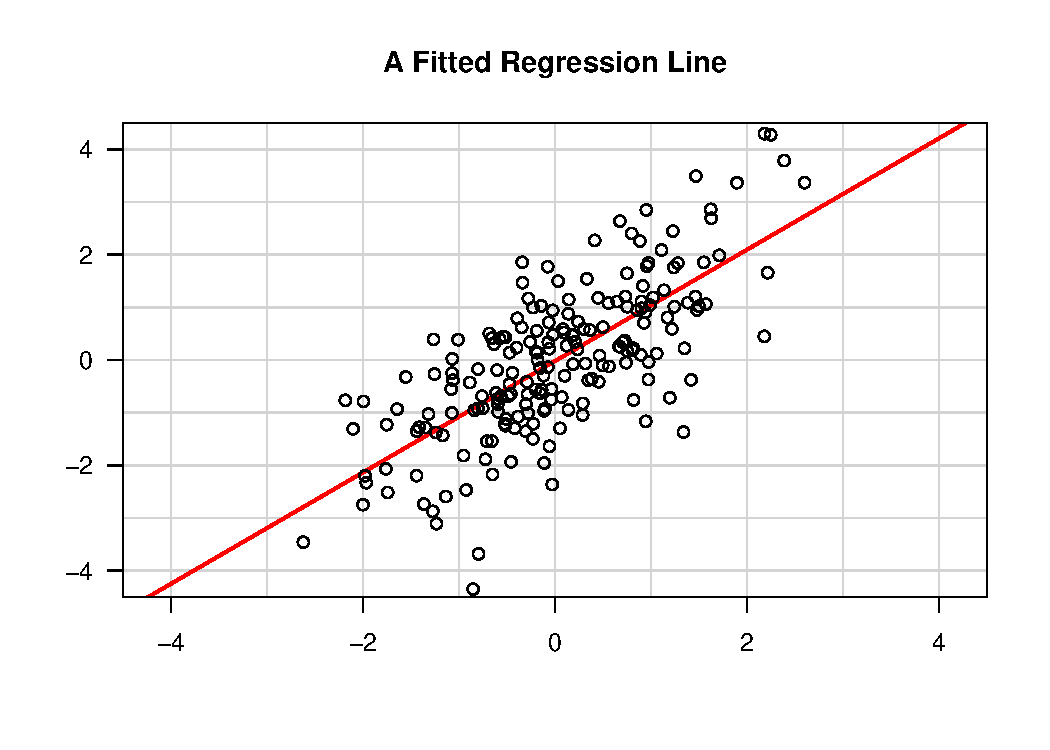
\includegraphics[width=.9\linewidth,height=.7\linewidth]{figure/ablines-1} 

}



\end{knitrout}
\end{frame}

%------------------------------------------------

\begin{frame}[fragile]
\frametitle{Creating a Plot from Scratch}

\bbi
  \item Start a new plot with \code{plot.new()}
  \item \code{plot.new()} opens a new (empty) plot frame
  \item \code{plot.new()} chooses a default plotting region
\ei

\end{frame}

%------------------------------------------------

\begin{frame}[fragile]
\frametitle{Setting Up Coordinates}

Then use \code{plot.window()} to set up the coordinate system for the plotting frame
\begin{knitrout}\footnotesize
\definecolor{shadecolor}{rgb}{0.969, 0.969, 0.969}\color{fgcolor}\begin{kframe}
\begin{alltt}
\hlcom{# axis limits (0,1)x(0,1)}
\hlkwd{plot.window}\hlstd{(}\hlkwc{xlim} \hlstd{=} \hlkwd{c}\hlstd{(}\hlnum{0}\hlstd{,} \hlnum{1}\hlstd{),} \hlkwc{ylim} \hlstd{=} \hlkwd{c}\hlstd{(}\hlnum{0}\hlstd{,} \hlnum{1}\hlstd{))}
\end{alltt}
\end{kframe}
\end{knitrout}
By default \code{plot.window()} produces axis limits which are expanded by 6\% over those actually specified. 

\end{frame}

%------------------------------------------------

\begin{frame}[fragile]
\frametitle{Setting Up Coordinates}

The default limits expansion can be turned-off by specifying \code{xaxs = "i"} and/or \code{yaxs = "i"}
\begin{knitrout}\footnotesize
\definecolor{shadecolor}{rgb}{0.969, 0.969, 0.969}\color{fgcolor}\begin{kframe}
\begin{alltt}
\hlkwd{plot.window}\hlstd{(xlim, ylim,} \hlkwc{xaxs} \hlstd{=} \hlstr{"i"}\hlstd{)}
\end{alltt}
\end{kframe}
\end{knitrout}

\end{frame}

%------------------------------------------------

\begin{frame}[fragile]
\frametitle{Aspect Ratio Control}

Another important argument is \code{asp}, which allows us to specify the \textbf{aspect ratio}
\begin{knitrout}\footnotesize
\definecolor{shadecolor}{rgb}{0.969, 0.969, 0.969}\color{fgcolor}\begin{kframe}
\begin{alltt}
\hlkwd{plot.window}\hlstd{(xlim, ylim,} \hlkwc{xaxs} \hlstd{=} \hlstr{"i"}\hlstd{,} \hlkwc{asp} \hlstd{=} \hlnum{1}\hlstd{)}
\end{alltt}
\end{kframe}
\end{knitrout}

\code{asp = 1} means that unit steps in the x and y directions produce equal distances in the x and y directions on the plot.
(Important to avoid distortion of circles that
look like ellipses)

\end{frame}

%------------------------------------------------

\begin{frame}[fragile]
\frametitle{Drawing Axes}

The \code{axis()} function can be used to draw axes at any of the four sides of a plot.
\bi
  \item \code{side=1} below the graph
  \item \code{side=2} to the left of the graph
  \item \code{side=3} above the graph
  \item \code{side=4} to the right of the graph
\ei

\end{frame}

%------------------------------------------------

\begin{frame}[fragile]
\frametitle{Customizing Axes}

Axes can be customized via several arguments (see \code{?axis})
\bi
  \item location of tick-marks
  \item labels of axis
  \item colors
  \item sizes
  \item text fonts
  \item text orientation 
\ei

\end{frame}

%------------------------------------------------

\begin{frame}
\frametitle{Plot Annotation}

The function \code{title()} allows us to include labels in the margins
\bi
  \item \code{main} main title above the graph
  \item \code{sub} subtitle below the graph
  \item \code{xlab} label for the x-axis
  \item \code{ylab} label for the y-axis
\ei

\end{frame}

%------------------------------------------------

\begin{frame}
\frametitle{Customizing Annotations}

The annotations can be customized with additional arguments for the fonts, colors, and size (expansion)
\bi
  \item \code{font.main, col.main, cex.main} 
  \item \code{font.sub, col.sub, cex.sub}
  \item \code{font.lab, col.lab, cex.lab}
\ei

\end{frame}

%------------------------------------------------

\begin{frame}[fragile]
\frametitle{Drawing Arrows}

Arrows can be drawn with the function:
\begin{verbatim}
arrows(x0, y0, x1, y1, code = int, 
       length = num, angle = num)
\end{verbatim}

\bi
  \item The \code{x0, y0, x1, y1} arguments give the start and end coordinates.
  \item \code{code=1} head at the start, \code{code=2} head at the end, \code{code=3} head at both ends
  \item \code{length} of the arrow head and \code{angle} to the shaft
\ei

\end{frame}

%------------------------------------------------

\begin{frame}[fragile]
\frametitle{Drawing Arrows}
\begin{knitrout}\footnotesize
\definecolor{shadecolor}{rgb}{0.969, 0.969, 0.969}\color{fgcolor}\begin{kframe}
\begin{alltt}
\hlkwd{plot.new}\hlstd{()}
\hlkwd{plot.window}\hlstd{(}\hlkwc{xlim} \hlstd{=} \hlkwd{c}\hlstd{(}\hlnum{0}\hlstd{,} \hlnum{1}\hlstd{),} \hlkwc{ylim} \hlstd{=} \hlkwd{c}\hlstd{(}\hlnum{0}\hlstd{,} \hlnum{1}\hlstd{))}
\hlkwd{arrows}\hlstd{(}\hlnum{.05}\hlstd{,} \hlnum{.075}\hlstd{,} \hlnum{.45}\hlstd{,} \hlnum{.9}\hlstd{,} \hlkwc{code} \hlstd{=} \hlnum{1}\hlstd{)}
\hlkwd{arrows}\hlstd{(}\hlnum{.55}\hlstd{,} \hlnum{.9}\hlstd{,} \hlnum{.95}\hlstd{,} \hlnum{.075}\hlstd{,} \hlkwc{code} \hlstd{=} \hlnum{2}\hlstd{)}
\hlkwd{arrows}\hlstd{(}\hlnum{.1}\hlstd{,} \hlnum{0}\hlstd{,} \hlnum{.9}\hlstd{,} \hlnum{0}\hlstd{,} \hlkwc{code} \hlstd{=} \hlnum{3}\hlstd{)}
\hlkwd{text}\hlstd{(}\hlnum{.5}\hlstd{,} \hlnum{1}\hlstd{,} \hlstr{"A"}\hlstd{,} \hlkwc{cex} \hlstd{=} \hlnum{1.5}\hlstd{)}
\hlkwd{text}\hlstd{(}\hlnum{0}\hlstd{,} \hlnum{0}\hlstd{,} \hlstr{"B"}\hlstd{,} \hlkwc{cex} \hlstd{=} \hlnum{1.5}\hlstd{)}
\hlkwd{text}\hlstd{(}\hlnum{1}\hlstd{,} \hlnum{0}\hlstd{,} \hlstr{"C"}\hlstd{,} \hlkwc{cex} \hlstd{=} \hlnum{1.5}\hlstd{)}
\end{alltt}
\end{kframe}
\end{knitrout}
\end{frame}

%------------------------------------------------

\begin{frame}[fragile]
\frametitle{Drawing Arrows}
\begin{knitrout}\scriptsize
\definecolor{shadecolor}{rgb}{0.969, 0.969, 0.969}\color{fgcolor}

{\centering 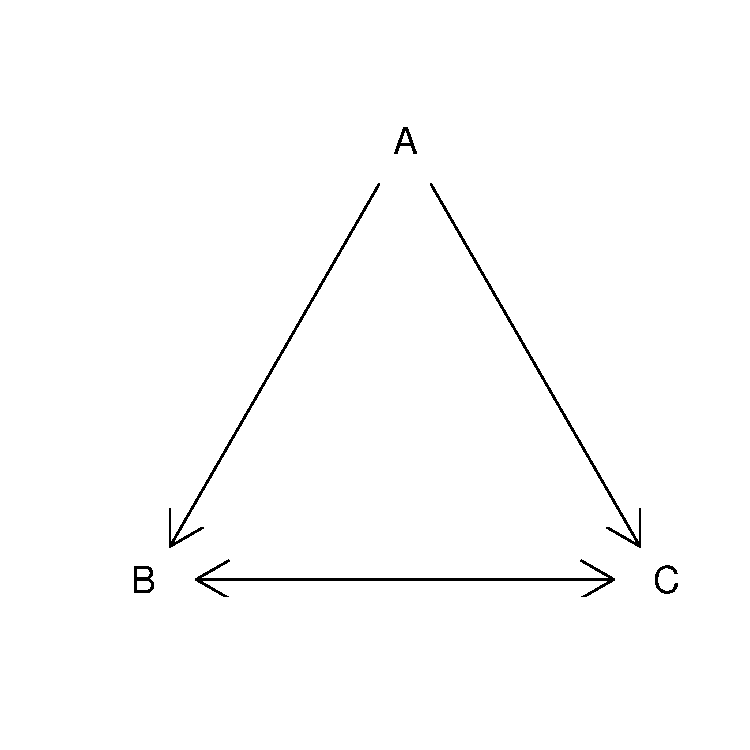
\includegraphics[width=.8\linewidth,height=.8\linewidth]{figure/arrows-1} 

}



\end{knitrout}
\end{frame}

%------------------------------------------------

\begin{frame}[fragile]
\frametitle{Drawing Rectangles}

Rectangles can be drawn with the function:
\begin{verbatim}
rect(x0, y0, x1, y1, col = str, border = str)
\end{verbatim}

\bi
  \item \code{x0, y0, x1, y1} give the coordinates of diagonally opposite corners of the rectangles.
  \item \code{col} specifies the color of the interior.
  \item \code{border} specifies the color of the border.
\ei

\end{frame}

%------------------------------------------------

\begin{frame}[fragile]
\frametitle{Drawing Rectangles}
\begin{knitrout}\footnotesize
\definecolor{shadecolor}{rgb}{0.969, 0.969, 0.969}\color{fgcolor}\begin{kframe}
\begin{alltt}
\hlcom{# barplot manually constructed}
\hlkwd{plot.new}\hlstd{()}
\hlkwd{plot.window}\hlstd{(}\hlkwc{xlim} \hlstd{=} \hlkwd{c}\hlstd{(}\hlnum{0}\hlstd{,} \hlnum{5}\hlstd{),} \hlkwc{ylim} \hlstd{=} \hlkwd{c}\hlstd{(}\hlnum{0}\hlstd{,} \hlnum{10}\hlstd{))}
\hlkwd{rect}\hlstd{(}\hlnum{0}\hlopt{:}\hlnum{4}\hlstd{,} \hlnum{0}\hlstd{,} \hlnum{1}\hlopt{:}\hlnum{5}\hlstd{,} \hlkwd{c}\hlstd{(}\hlnum{7}\hlstd{,} \hlnum{8}\hlstd{,} \hlnum{4}\hlstd{,} \hlnum{3}\hlstd{),}
     \hlkwc{col} \hlstd{=} \hlstr{"turquoise"}\hlstd{,}
     \hlkwc{border} \hlstd{=} \hlstr{"white"}\hlstd{)}
\hlkwd{axis}\hlstd{(}\hlnum{1}\hlstd{)}
\hlkwd{axis}\hlstd{(}\hlnum{2}\hlstd{,} \hlkwc{las} \hlstd{=} \hlnum{1}\hlstd{)}
\end{alltt}
\end{kframe}
\end{knitrout}
\end{frame}

%------------------------------------------------

\begin{frame}[fragile]
\frametitle{Drawing Rectangles}
\begin{knitrout}\scriptsize
\definecolor{shadecolor}{rgb}{0.969, 0.969, 0.969}\color{fgcolor}

{\centering 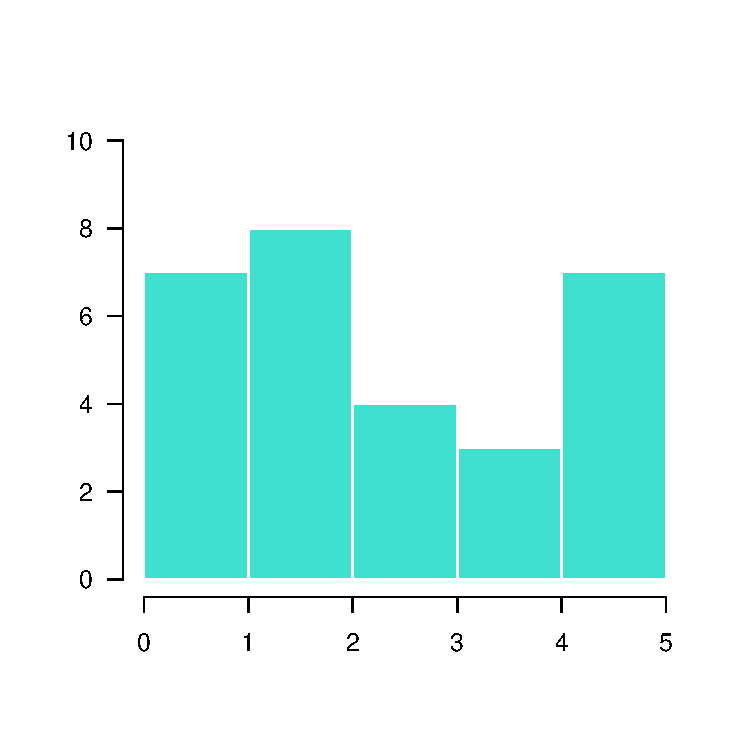
\includegraphics[width=.8\linewidth,height=.8\linewidth]{figure/rectangles-1} 

}



\end{knitrout}
\end{frame}

%------------------------------------------------

\begin{frame}
\begin{center}
\Huge{\hilit{Plot Regions}}
\end{center}
\end{frame}

%------------------------------------------------

\begin{frame}
\frametitle{Anatomy of Plot Frame and Region}
\begin{center}
\ig[width=6cm]{images/plot_region.pdf}
\end{center}
\end{frame}

%------------------------------------------------

\begin{frame}[fragile]
\frametitle{Adjusting the Margins}

Margins can be adjusted with the \code{par()} function in various ways:
\bi
  \item In inches: \code{par(mai = c(2, 2, 1, 1))}
  \item In lines of text: \code{par(mar = c(4, 4, 2, 2))}
  \item Width and Height in inches: \code{par(pin = c(5, 4))}
\ei

\end{frame}

%------------------------------------------------

\begin{frame}[fragile]
\frametitle{One more scatter plot}
\begin{knitrout}\footnotesize
\definecolor{shadecolor}{rgb}{0.969, 0.969, 0.969}\color{fgcolor}\begin{kframe}
\begin{alltt}
\hlcom{# simple scatter-plot}
\hlstd{op} \hlkwb{<-} \hlkwd{par}\hlstd{(}\hlkwc{mar} \hlstd{=} \hlkwd{c}\hlstd{(}\hlnum{5}\hlstd{,} \hlnum{4}\hlstd{,} \hlnum{3}\hlstd{,} \hlnum{1}\hlstd{))}
\hlkwd{plot}\hlstd{(mtcars}\hlopt{$}\hlstd{mpg, mtcars}\hlopt{$}\hlstd{hp,} \hlkwc{type} \hlstd{=} \hlstr{"n"}\hlstd{,}
     \hlkwc{xlab} \hlstd{=} \hlstr{"miles per gallon"}\hlstd{,} \hlkwc{ylab} \hlstd{=} \hlstr{"horsepower"}\hlstd{)}
\hlcom{# grid lines}
\hlkwd{abline}\hlstd{(}\hlkwc{v} \hlstd{=} \hlkwd{seq}\hlstd{(}\hlkwc{from} \hlstd{=} \hlnum{10}\hlstd{,} \hlkwc{to} \hlstd{=} \hlnum{30}\hlstd{,} \hlkwc{by} \hlstd{=} \hlnum{5}\hlstd{),} \hlkwc{col} \hlstd{=} \hlstr{'gray'}\hlstd{)}
\hlkwd{abline}\hlstd{(}\hlkwc{h} \hlstd{=} \hlkwd{seq}\hlstd{(}\hlkwc{from} \hlstd{=} \hlnum{50}\hlstd{,} \hlkwc{to} \hlstd{=} \hlnum{300}\hlstd{,} \hlkwc{by} \hlstd{=} \hlnum{50}\hlstd{),} \hlkwc{col} \hlstd{=} \hlstr{' gray'}\hlstd{)}
\hlcom{# points}
\hlkwd{points}\hlstd{(mtcars}\hlopt{$}\hlstd{mpg, mtcars}\hlopt{$}\hlstd{hp,} \hlkwc{pch} \hlstd{=} \hlnum{19}\hlstd{,} \hlkwc{col} \hlstd{=} \hlstr{"blue"}\hlstd{)}
\hlcom{# text (point labels)}
\hlkwd{text}\hlstd{(mtcars}\hlopt{$}\hlstd{mpg, mtcars}\hlopt{$}\hlstd{hp,} \hlkwc{labels} \hlstd{=} \hlkwd{rownames}\hlstd{(mtcars),}
     \hlkwc{pos} \hlstd{=} \hlnum{4}\hlstd{,} \hlkwc{col} \hlstd{=} \hlstr{"gray50"}\hlstd{)}
\hlcom{# title}
\hlkwd{title}\hlstd{(}\hlstr{"Miles Per Galon -vs- Horsepower"}\hlstd{)}
\hlcom{# reset graphical margins}
\hlkwd{par}\hlstd{(op)}
\end{alltt}
\end{kframe}
\end{knitrout}
\end{frame}

%------------------------------------------------

\begin{frame}[fragile]
\begin{knitrout}\footnotesize
\definecolor{shadecolor}{rgb}{0.969, 0.969, 0.969}\color{fgcolor}

{\centering 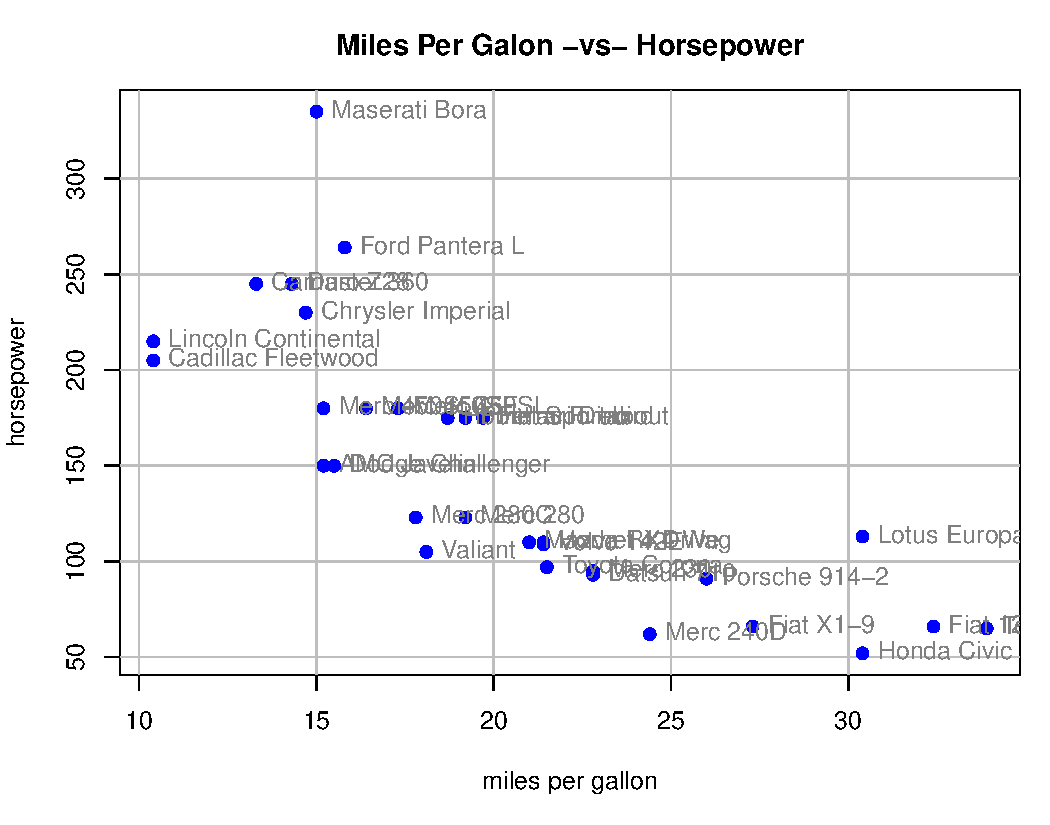
\includegraphics[width=.8\linewidth,height=.7\linewidth]{figure/margins_plot-1} 

}



\end{knitrout}
\end{frame}

%------------------------------------------------


\end{document}
